\documentclass[12pt]{article}

% add some essential packages, some might not be used
%\usepackage{CJKutf8}
\usepackage[T1]{fontenc}
\usepackage[utf8]{inputenc}
\usepackage[usenames,dvipsnames]{color}
\usepackage{authblk}
\usepackage{xeCJK}
\usepackage{ragged2e}
\usepackage{amsmath}
%\usepackage[a4paper,margin=2in,bottom=1.0in]{geometry}
\usepackage{url}
\usepackage{array}
\usepackage{bbding}
\usepackage{amssymb}
\usepackage{graphicx}
\usepackage{adjustbox}
\usepackage{subcaption}
\usepackage{caption}
\usepackage{booktabs}
\usepackage{float}
\usepackage{appendix}
\usepackage{url}
\usepackage[english]{babel}
\usepackage{adjustbox}
\usepackage{textgreek}
\usepackage{NotesTeX}
\usepackage{lipsum}
\usepackage[procnames]{listings}
\usepackage{wasysym}
\usepackage{amsthm}
\usepackage{framed}
\usepackage[procnames]{listings}
\usepackage[scaled=0.9]{DejaVuSansMono}
\usepackage{pythonhighlight}
%\usepackage{marvosym} % coffeecup 

\usepackage[ruled,vlined]{algorithm2e}

\usepackage{rotating} % for the horizontal page table

\usepackage{tikz}
\usetikzlibrary{calc}
\usetikzlibrary{matrix}
\usetikzlibrary{positioning}
\usepackage{color}
\usepackage{setspace}
% python highlight package
\usepackage{pifont} % checkmark package 

\newcommand{\zn}{\mathbb{Z}}
\newcommand{\cn}{\mathbb{C}}
\newcommand{\qn}{\mathbb{Q}}
\newcommand{\rn}{\mathbb{R}}
\newcommand{\pn}{\mathbb{P}}
\newcommand{\fn}{\mathbb{F}}
\newcommand{\nn}{\mathbb{N}}

\numberwithin{figure}{section}

\usepackage{tcolorbox} % package for making colorful box

 \setlength{\parskip}{0.15cm} % change the paragraph spacing
\renewcommand\labelitemi{$\vcenter{\hbox{\tiny$\bullet$}}$} % set the bullet size as tiny

% \newcommand*\rot{\rotatebox{90}} % for rotate text

%\usepackage{courier}

\newenvironment{fullmodel}{
			\smallskip\noindent
			\begin{minipage}{\textwidth+\marginparwidth+\marginparsep}\smallskip\smallskip}
			{\smallskip\smallskip\end{minipage}\vspace{.1in}
			}



\title{{\Huge 人工智能基础(高中版)}\\{\Large{辅导讲义}}}
\author{王斐 Michael\footnote{\href{https://www.michaelyunfei.com}{\textit{Author Website}}}}

\affiliation{Team of Education, SenseTime}
\emailAdd{michael.yunfei@gmail.com}


\numberwithin{equation}{section}



\newenvironment{question}[2][Question]{\begin{trivlist}
\item[\hskip \labelsep {\bfseries #1}\hskip \labelsep {\bfseries #2.}]}{\end{trivlist}}

\setcounter{tocdepth}{2}

\begin{document}
  \maketitle
  \flushbottom
  \newpage
  \pagestyle{fancynotes}

\definecolor{franceblue}{RGB}{156, 195, 228}
\definecolor{medblue}{RGB}{88, 157, 196}




%\setcounter{part}{}


\part*{第一章: 何谓机器学习}

同学们如果已经阅读过教材第一章,或者观看过有关人工智能的相关介绍视频的话,那么应该会对人工智能有一定的了解。在过去几年里,人工智能领域新的方法和应用层出不穷,可谓`发展神速'。目前人工智能的应用主要依赖的是机器学习\sn{Machine Learning}和深度学习\sn{Deep Learning}中的模型。而这些模型之所以能够引起全社会的重视(大到国家政策,小到学校教育),是因为在大数据的时代,机器学习所引发的是一场\textbf{思维转换运动}。那么这一章节,我们将会重点剖析何谓机器学习,已经它又将引发怎样的思维范式转变。


在本章的整个学习过程中,我希望同学们可以思考下面几个问题\mn{这几个问题是我们课程的核心中的核心,所以希望同学们倍加留意}。

\begin{tcolorbox}[title=本章思考问题]
	人工智能依赖得是机器学习模型,那么请同学们思考:
	\begin{itemize}
		\item 什么是`学习'?
		\item 人类如何`学习'?
		\item 机器如何`学习'?
	\end{itemize}
\end{tcolorbox}

这些问题较为抽象,我给同学们提供几个思路。我们汉语中,`学'是从受教和觉悟延伸而来,`学’意味着受教的过程,比如我们会说`我从妈妈那里学会了做饭', 或者`我从老师那里学习了人工智能的模型'。汉字`学’在英文中即对应`learn',也对应`study'\mn{但是在英文中 learn 更注重生活知识和技能的获取,而study更强调学院内容和专业素养的培训。比如, I learn how to cook from my parents, I study economics at univerity.}。 简单概括,我们可以说`学'是一个积累知识和技能的过程。

那么`习’顾名思义更多得意味`练习'. 我们在获取了任何一种知识和技能的话,如果想要加深理解并且进一步应用,那么就需要不断练习。我们经常说,每个人成长的过程就是不断学习的过程,我们从一开始得蹒跚步履,到现在红绿灯、楼宇、交通得灵活穿梭,背后都是一点一滴得学和习的过程。\marginnote{\begin{tcolorbox}[colframe=gray]如果同学们坐下来想一想自己成长到现在所学习的知识和技能的话,每一个人都应该为自己而骄傲,并为可以成为万物灵长的人而微暖。\end{tcolorbox}}

与人类的\textbf{综合学习}能力来对比,目前计算机在人工智能领域的发展还处于很初级得阶段,也就是说:\textbf{计算机目前只能对单一问题在有规律呈现的基础上进行学习}。但是考虑到人类是喜欢追求规律和创造规律的社会性动物,所以即使计算机只能对单一问题在有规律呈现的基础上学习的话,那么它所带来的改变也很有可能会是超乎想象得。但是稍安勿躁, 我们还是来认真探讨下什么是\textbf{机器学习},以及机器是如何学习的。


\setcounter{section}{1}
\subsection{课前预习C1}

为了提高沟通速率且帮助同学们养成良好学习节奏,我们以后会将课前预习,课上笔记,及课后练习简称为C1, C2, C3。比如,如果我说\textit{`你需要在下周一之前完成C1',那就意味着你需要根据我在C1中的指示进行课前预习}。下面的表格是后面课程中C1, C2, C3中的包含的内容以及所设定的预订目标。

\begin{table}[H]
	\centering
	\renewcommand{\arraystretch}{1.6}
	\begin{tabular}{|c|c|c|c|}
		\hline
		& C1 & C2 & C3 \\
		\hline 
		主题& 背景资料阅览 & 课堂老师讲解 & 课后习题和编程 \\
		\hline
		内容& 生活常识回顾 & 辅导讲义和课件 & 数学练习和Python练习 \\
		\hline
		时长 & 30分钟-1小时 & 45分钟 & 2-3 小时 \\
		\hline 
		频率 & 一周一次 & 一周三次 & 一周一次 \\
		\hline 
		 & \checkmark & \multicolumn{2}{c|}{只完成C1好比看了一场有关AI的电影} \\
		\cline{2-4}
		收获&  \checkmark & \checkmark & 不作习题C2完全是浪费时间 \\
		\cline{2-4}
		& \checkmark & \checkmark & \checkmark C1-C3全部完成可以得A+ \\
		\hline 
	\end{tabular}
\end{table}


这一节课的课前预习有两个部分:
\begin{itemize}
	\item 小作文(60字)
	\item 异常简单得解方程题目和一个游戏设计题目
\end{itemize}

\noindent
\textit{第一部分: 小作文}

请同学们选取一个学习过程,可以是学习做饭,学习解答数学题目,学习吉他等等,然后在60字内总结你的学习流程,该学习流程需要包涵以下三个环节:
\begin{enumerate}
	\item 哪里获取得知识和信息(比如,从父母,从老师,从网络等)
	\item 获得了这些知识和信息后你是如何理解的
	\item 学过之后是怎样练习的
\end{enumerate}


\noindent
\textit{第二部分: 课前小习题}

这些课前小习题虽然非常简单,但是其所包含的思想和具体的启示非常重要。所以希望同学们按时完成,并且在上课前将答案准备好。


\begin{question}{C1-Q1}
已知下列一组方程,求解$x$ 和$y$的值: 
\begin{align*}
	2x + 3y & = 9 \\
	x -2y & = 1
\end{align*}	
\end{question}


\begin{question}{C1-Q2}
	已知下列方程,请给$x$ 和 $y$ 赋值从而可以使得方程成立(为真):
	\begin{align*}
		x + 2y = 6 
	\end{align*}
	并思考有多少个$x$和$y$的选项可以使得上述方程成立?
\end{question}



\begin{question}{C1-Q3}
	已知下列方程组,请问可以求解$x, y, z$吗?如果可以,为什么?如果不可以,为什么?
	\begin{align*}
		2x + 3y + z & =9 \\
		x - 2y + 3z & = 16
	\end{align*}
\end{question}

\noindent



\begin{question}{C1-Q4}
在C1-Q2中我们有以下方程组
\begin{align*}
	2x + 3y & = 9 \\
	x -2y & = 1
\end{align*}	
现在我们将以上方程组,重新组织下\textbf{呈现方式},表现我下面的形式:
\begin{align*}
	\begin{bmatrix}
	2 & 3 \\
	1 & -2 
\end{bmatrix} \begin{bmatrix}
	x \\
	y 
\end{bmatrix} = \begin{bmatrix}
	9 \\
	1 
\end{bmatrix} \tag{形式1}
\end{align*}
我们也可以把他们放到一张表格中去
\begin{table}[H]
	\centering
	\begin{tabular}{|c|c|c|}
	\hline 
		x & y & 结果 \\
		\hline 
		2 & 3 & 9 \\
		1 & -2 & 1 \\
		\hline 
	\end{tabular}
\end{table}
按照以上格式,将C1-Q3中的方程组写成形式1和表格。
\end{question}



\begin{question}{C1-Q5}
	(游戏设计)随意选取一个任意的方程(优选简单一点的方程), 比如$f(x) = x + x^2$,然后根据你选择的方程完成下列表格(计算$f(x)$的值,可以用计算器):
	\begin{table}[H]
		\centering
		\begin{tabular}{|c|cccccccc|}
		\hline 
			方程 & \multicolumn{7}{l}{$f(x)=$} &  \\
			\hline 
			 x & 1 & 2 & 3 & 4 & 5 & 6 & 7 & 8 \\
			 \hline 
			 $f(x)$ & & & & & & & & \\
			 \hline 
		\end{tabular}
	\end{table}
\end{question}




\textcolor{purple}{反馈统计}:请扫描右边二维码,回答对此次课前预习的评估,只有三个问题。Michael 表示非常感谢,请同学多多配合。老师会根据你们的反馈对每一次C1进行提升和改进。填问卷的时候记得喝一杯茶或者咖啡$\heartsuit$。


\begin{marginfigure}
	\centering
	
\includegraphics[width=\textwidth]{fig/C1C1qrcode}
\end{marginfigure}


\begin{tcolorbox}[colback=white]
在正式进入本章的讲解之前,老师也想参与一下课前预习中C1-Q5的游戏设计题目。下面是老师选择的一个简单方程:
\begin{align*}
	f(x) = 2x - 1 
\end{align*}
根据该方程,我们可以得到以下表格
\begin{table}[H]
	\centering
	\begin{tabular}{cccccccccccc}
		\hline 
		x & 0 & 1 & 2 & 3 & 4 & 5 & 6 & 7 & 8 & 9 \\
		$f(x)$ & -1 & 1 & 3 &  5 &  7 &  9 & 11 &  13 & 15 & ? \\
		\hline 
	\end{tabular}
\end{table}
老师有选取了一个较为复杂的方程:
\begin{align*}
	f(x) = x^2 + 2x - 3 
\end{align*}
根据该方程,我们可以得到以下表格
\begin{table}[H]
	\centering
	\begin{tabular}{ccccccccccc}
		\hline 
		x & 1 & 2 & 3 & 4 & 5 & 6 & 7 & 8 & 9 \\
		$f(x)$ & 0 & 5 &  12 &  21 &  32 & 45 &  60 & 77 & 96 \\
		\hline 
	\end{tabular}
\end{table}
\end{tcolorbox}

\begin{fullmodel}
现在,我们上述第一个表格中$x = 0, 1, 2, \cdots, 8$, 以及$f(x)=-1, 1, 3, \cdots, 15$作为原始数据输入到一个简单的神经网络模型中,但是并不告诉计算机我们的方程公式,来看一下根据\textbf{已知的$x$和$f(x)$}, 计算机能否预测$f(x=9)$。下面是一个简单的神经网络模型的运行结果。
\begin{python}
import tensorflow as tf
from tensorflow import keras


def Learn_model(y_new):
    xs = np.array(range(0, 9), dtype=float)
    ys = np.array([-1.0, 1.0, 3.0, 5.0, 7.0, 9.0, 11.0, 13.0, 15.0], dtype=float)
    model = tf.keras.Sequential([keras.layers.Dense(units=1, input_shape=[1])])
    model.compile(optimizer='sgd', loss='mean_squared_error')
    model.fit(xs, ys, epochs=100)
    return model.predict(y_new)[0]


prediction = Learn_model([9.0])
print(prediction)  # 16.47 (70.97 for the second function)
\end{python} 	
我们看到简单的神经网络模型给出的预测值是 16.47 。虽然与我们的计算值 17 ,有一定差距,但是考虑到我们只给出了9个匹配数据组,模型(训练次数为100次)便可以预测出与真值相差不大的结果,这已经可以显示机器学习的魅力所在了。
\end{fullmodel}

\subsection{课堂讲义C2}

我们这一章\mn{课堂讲义里的内容是你应该重点学习的内容,学期末的考核所包含的知识点,都涵盖在课堂讲义中,所以你要做到`熟读百遍,而有备无患'。}的主题是:\textbf{何谓机器学习},所以学习重点便在于领会机器学习的框架。机器学习与传统的问题解决方法的最大不同,可以用下面这张图表(来源:Laurence Moroney)来形容。
\begin{figure}[H]
	\centering
	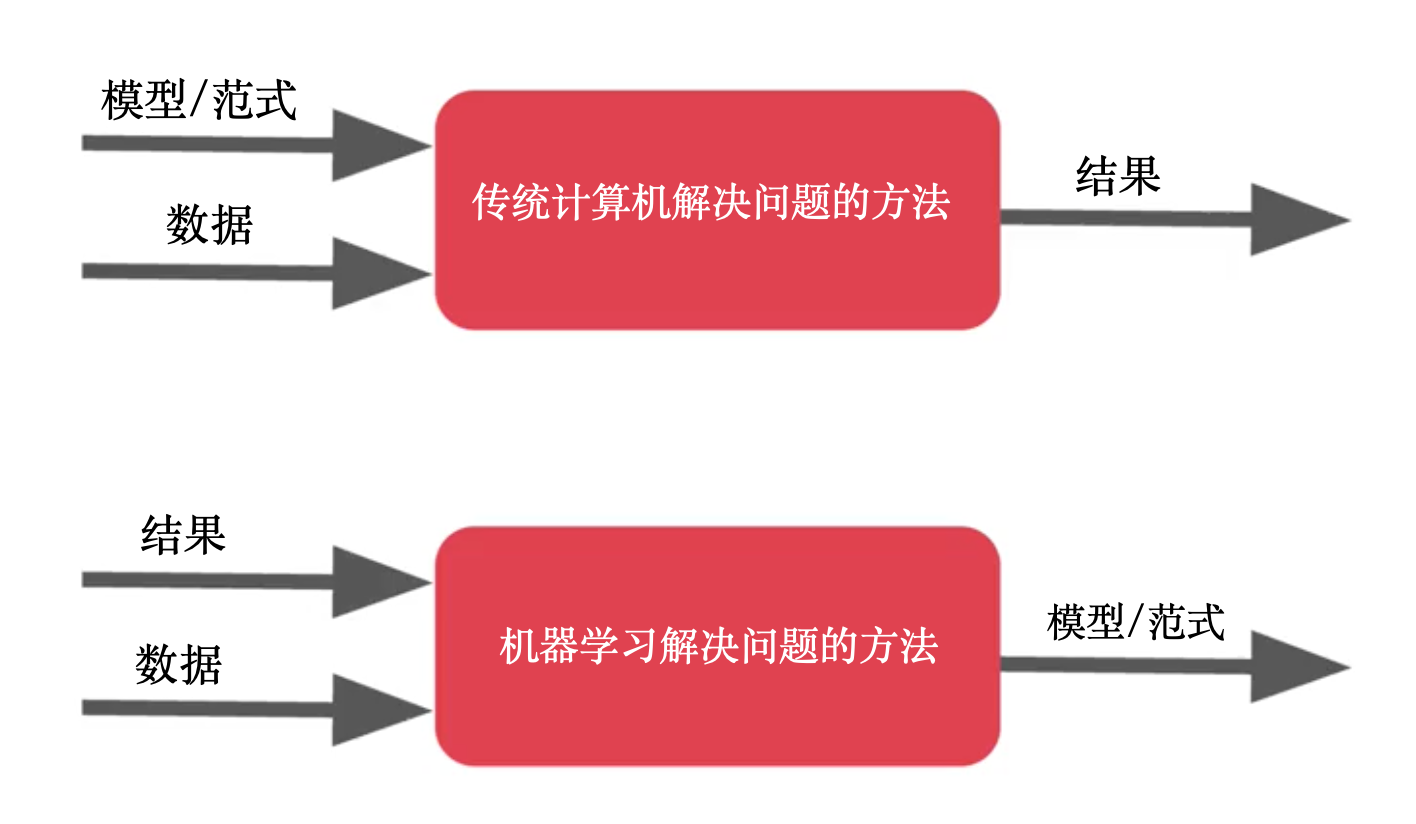
\includegraphics[width=0.65\textwidth]{fig/C1MLbigpct}
	\caption{机器学习解决问题的方法}
\end{figure}

在实际生活中,不同领域的专家会构建非常复杂的模型来解决不同的问题。但是传统的解决问题的思路都可以概括为:
\begin{itemize}
	\item 认识问题
	\item 对相关问题进行一般抽象,并且建立相关数理模型
	\item 根据模型编写程序
	\item 对程序进行测试后推广应用
\end{itemize}
比如船体工程师在对甲板的承压测试时,会考虑甲板的质料,外部化学环境,已经物理力学的一般定理,然后编写甲板的压力承受程序。根据已经写好的程序,当甲板受力过大时,就会发出警报。

但是机器学习的模型解决问题的方法则非常不同,总体可以概括为:
\begin{itemize}
	\item 收集大量数据(数据中包含了一定的规律)\mn{希望后面同学们能够理解为什么数据会变得越来越重要,或者能够体会机器学习模型下支撑的人工智能产业需要消耗大量数据的原因。}
	\item 将不同数据与去对应的结果一并输入
	\item 然后机器学习的模型会经过一定训练后学习数据背后的规律(或范式)
	\item 根据其学习到的这些规律来进行预测
\end{itemize}

\begin{fullmodel}
\begin{tcolorbox}[title=章节重点]
	我们这一章会围绕图1.1来深入得了解机器学习的理论大框架,并且帮助同学们建立\textbf{人工智能思维},所以希望同学们认真学习。去领会人工智能思维时,这一章会有下面三个小节:
	\begin{itemize}
		\item 为什么需要机器学习模型以及神经网络模型
		\item 机器学习解决问题的方法
		\item 人工智能思维原素
	\end{itemize}
注:我们还没有介绍任何具体的机器学习和神经网络模型,同学们会动第二章开始逐渐学习不同的模型。虽然只有在学习这些模型之后,才能更深入得领会人工智能思维,但是通过本章的学习,即使在没有了解任何机器学习或者神经网络模型前,你仍然可以体会何谓人工智能和机器学习。
\end{tcolorbox}
\end{fullmodel}


\subsubsection{为什么需要机器学习模型}

\begin{definition}
	\textbf{人工智能}指的是计算机(或者其它机器)在人的指导下可以具备与人类某一项智力相匹配的能力。比如,在人的指导和帮助下,计算机可以对不同的物体进行识别,在很多情况下计算机因为在电力的帮助下,其工作时长和工作效率会远超于人类。
\end{definition}

\begin{definition}
	\textbf{机器学习}\mn{由于人工智能领域发展迅速,从业者有时会把人工智能和机器学习相等同,在我们的学习过程中,人工智能指向的是一种能力和思维方式,而机器学习则更侧重在我们现在定义下的一门学科。}指的是计算机根据一定的\textit{算法}在有\textit{数据}的支持下完成\textit{某一规律}的学习,且对其所学习到规律进行自动化调整。
\end{definition}

\begin{remark}
在计算机科学和数学科学中,\textit{算法}指的是为计算机解决某一问题时所罗列得有严格规范的指令代码。	由于计算机只能读取其所认可的数据,所以我们将其所学习到的\textit{规律}称为\textit{规律参数},这些规律参数可以一串数组,也可以有文本标记的数组。
\end{remark}

因为机器学习需要大量的数据,所以非常有必要对数据结构进行定义和分类\mn{生活中最常见的数据形式应该是Excel表格。}。

\begin{definition}
	我们把由数字和对其的描述(有其根据)组成的信息形态,称为\textit{数据};我们将统一在一个描述下的数列,称为\text{数据集}; 有多个数据集构成的一系列数据,称为\textit{数据阵}。
\end{definition}
\begin{marginfigure}
	\centering
	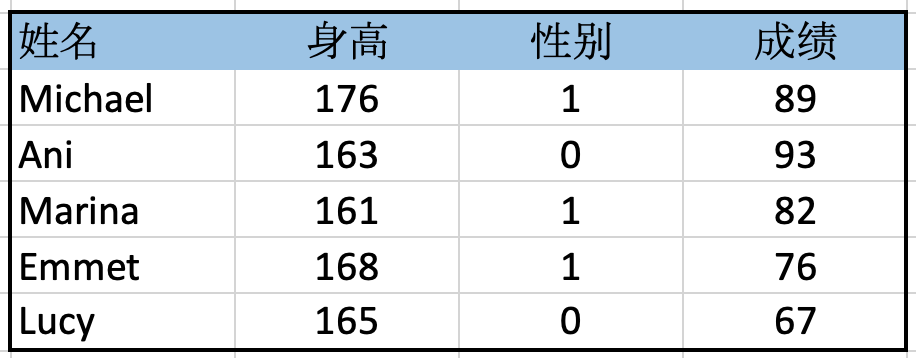
\includegraphics[width=0.9\textwidth]{fig/dataframeEx}
\end{marginfigure}
\begin{remark}
很显然,如果我只给你一个数,比如6, 我们不能称其为数据,因为其缺乏对其的描述。比如,`年方二八’, 年龄16岁,则可以成为数据。	再比如,2019 不是数据,2019年则是数据。
\end{remark}

\begin{example}
数据: 红色-255; 数据集: 颜色: 红255, 绿666, 蓝521; 数据阵:[[颜色:190, 321, 589]; [年份:2019, 2020, 2056]]。右边的表格就是一个数据阵。数据阵(dataframe)是Python和R语言中常用的数据形式。
\end{example}

\begin{definition}
	我们把语言文本,网页信息,图片和影音等的复合数据,称为\textit{多媒体数据集}。
\end{definition}

\begin{example}
下面这张图片是由 Peggy Collins 创作的马赛克数字图画。这张图片在计算机中的存储形式是具有维度$(1400, 1400, 3)$的数据集构成。其中3,是代表的RGB(红绿蓝)三层底色层,每一个色素层是由一个$1400 \times 1400$的矩阵组成。
\begin{figure}[H]
	\centering
	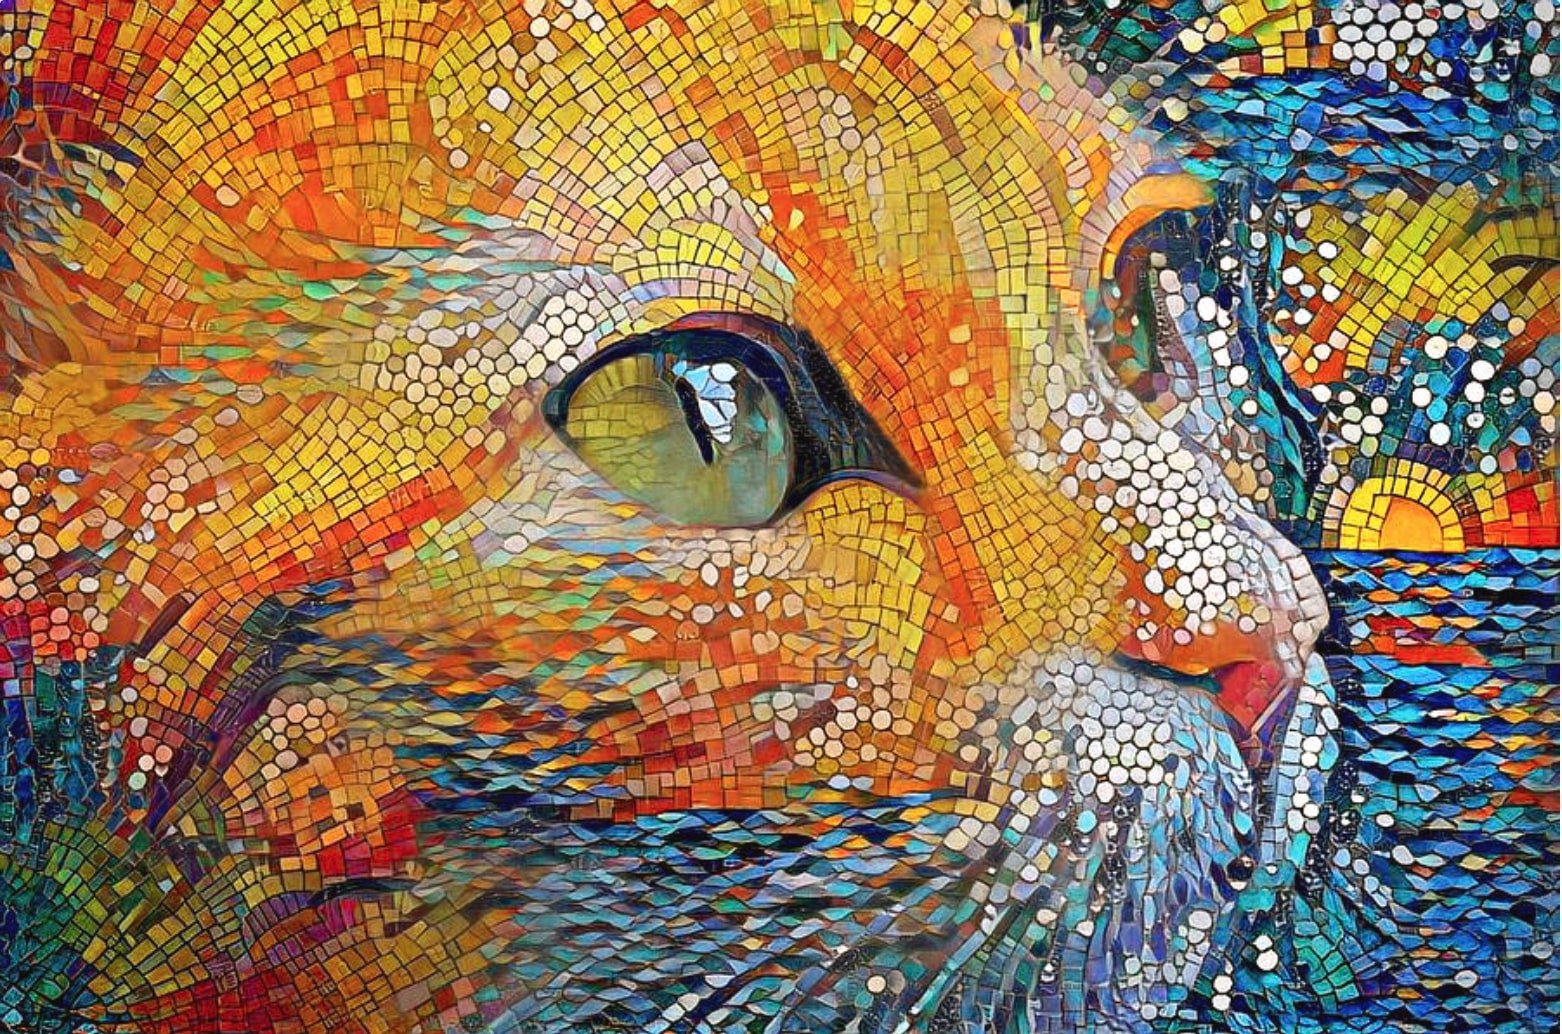
\includegraphics[width=\textwidth]{/Users/Michael/Documents/MDLforBeginners/Chapter3/Code/Images/Mosaic1.jpg}
	\caption{Ginger Cat by Peggy Collins (digital artwork)}
\end{figure}	
\begin{python}
print(im_mosaic1[:10, :10, 1])
# [[246 190 116  51  30  21   0   6  28  42]
#  [188  88  48  52  40  20   4  12  28  39]
#  [108  40  37  55  43  27  17  15  24  35]
#  [ 35  34  41  39  35  32  21  18  21  31]
#  [ 20  24  25  26  34  26  13  23  23  29]
#  [ 35  25  24  29  28  19  17  26  25  29]
#  [ 28  23  24  22  15  17  24  22  23  25]
#  [ 33  29  18  15  18  17  15  12  18  19]
#  [ 18  14  13  16  19  19  19  18  15  11]
#  [  8   6   8  16  23  26  24  21  20  15]]	
\end{python}
\end{example}

\begin{definition}
	我们将多媒体数据集和数据阵组合构成的数据形态成为\textit{数据群}或者\textit{大数据}。数据群或大数据,在业界也被称为\textbf{有标注的数据群}。
\end{definition}

\begin{example}
比如,下面这个表格是一个数据群的片段截取:\mn{大数据时代,数据的标注准确度和密集度,成为衡量数据群质量的重要指标。国际上,目前美国的数据群质量最高,其次是英国和德国。中国的数据群目前取胜于量,对于质的追求,还需要一定的时间。}
\begin{table}[H]
	\centering
	\renewcommand{\arraystretch}{1.5}
	\begin{tabular}{ccccc}
	\hline 
		图片(1400, 1400, 3) & 年份 & 地点 & 备注1 & 备注2 \\
		\hline 
		图1 & 2016 & 桥 & 青岛 & 红色 \\
		图2 & 2020 &  伦敦 & 人 & 女 \\
		图3 & 2013 & 成都& 熊猫 & 国宝\\
		\hline 
	\end{tabular}
\end{table}
\end{example}

\begin{fullmodel}
\begin{tcolorbox}[title={掌握基本术语后的`飞翔’}]
	在知道了什么是人工智能,机器学习以及相关的数据术语后,我们接下来就可以仔细探讨\underline{为什么需要机器学习模型了}。在开始之前,希望提醒同学们再回顾下相关的概念:
	\begin{itemize}
		\item 什么是机器学习?(最好再读一遍定义)
		\item 什么是数据?(数和数据的区别是什么)
		\item 什么是算法?
	\end{itemize}
\end{tcolorbox}
\end{fullmodel}

在课前预习中,我要求同学们解答一个二元方程组。我想同学们从初中开始就已经熟练掌握了这些问题。那么非常棒,只要你能解答二元方程组,那么我可以说你已经是半个机器学习专家了,因为虽然机器学习的模型可以很复杂,但是归根结底是一个代数方程问题。下面,我们就来解答一个较为难一点的方程组:
\begin{align*}
	& 56x + 8 y = 36 \\
	& 32 x + 4 y + z = 20.5 \\
	& 48 x + 3y + z = 29.8 
\end{align*}

经过的简单的计算你很快就可以得出:
\begin{align*}
	x = 0.6, y = 0.3, z = 0.1 
\end{align*}

\begin{example}
请问,如果我只给你一个方程:
\begin{align*}
	56x + 8y = 36 
\end{align*}	
你可以求出\textit{具体的}$x$和$y$值吗?实际上,如果只有一个方程的话,我们可以用无穷个解,比如$x=2, y = -9.5$。你可以用Python在进行快速计算。
\begin{python}
def c1c2fun1(x):
    """
    解方程 56x + 8y = 36
    输入: x
    输出: y
    """
    y = (36-56*x)/8

    return y
    

print(c1c2fun1(np.array(range(0, 8))))
# [ 4.5 -2.5  -9.5 -16.5 -23.5 -30.5 -37.5 -44.5]
\end{python}
\end{example}

\begin{example}
如果,我只给你两个方程, 你可以求解$x, y, z$ 吗?
\begin{align*}
	& 56x + 8 y = 36 \\
	& 32 x + 4 y + z = 20.5 
\end{align*}
我们知道,三个未知数需要三个方程组,很显然我们不能得到具体的解。(但是可以有无数解)
\end{example}

\begin{example}
现在我给你三个方程,但是第四个是由第二个两边同时乘以$2$得出的 $2 \times ( 32x + 4y + z) = 20.5 \times 2$
现在四个方程为:
\begin{align*}
	& 56x + 8 y = 36 \\
	& 32 x + 4 y + z = 20.5 \\
	& 64x + 8y + 2z = 41 
\end{align*}
你可以求解吗?。那下面这四个呢?
\begin{align*}
	& 56x + 8 y = 36 \\
	& 32 x + 4 y + z = 20.5 \\
	& 48 x + 3y + z = 29.8  \\
	& 59 x + 10y + z = 38.5
\end{align*}
\end{example}

我想同学们,肯定很轻松得就可以得出以下的规律:
\begin{itemize}
	\item 方程个数等于或大于未知变量个数时可能有具体解,也可能无具体解,取决于独立方程的个数。
	\item 方程个数小于未知变量个数时可以有无数的组合解
\end{itemize}


现在我们就把上面的方程组问题规范化,并且转换下表达形式。首先,我们将其表现矩阵和向量相乘的方式:
\begin{align*}
	\begin{bmatrix}
		56 & 8 & 0 \\
		32 & 4 & 1 \\
		48 & 3 & 1 
	\end{bmatrix} \begin{bmatrix}
		x \\
		y \\
		z 
	\end{bmatrix} = \begin{bmatrix}
		36 \\
		20.5 \\
		29.8 
	\end{bmatrix}
\end{align*}
其次我们也可以把这个方程组,表现为表格\mn{如果有同学不习惯新的术语,那么每次你在提到表格时,我们会默认其为数据阵。}形式,也就是我们所定义过的\textit{数据阵}形式:
\begin{table}[H]
	\centering
	\begin{tabular}{cccc}
	\hline 
		x & y & z & \\
		\hline 
		56 & 8 & 0 & 36 \\
		32 & 4 & 1 & 20.5 \\
		48 & 3 & 1 & 29.8 \\
		\hline 
	\end{tabular}
\end{table}

以上方程组或数据阵实际上一个现实生活中的案例截取。该案例描述得是不同学生学习状态和其成绩的统计,如下图显示。
\begin{figure}[H]
	\centering
	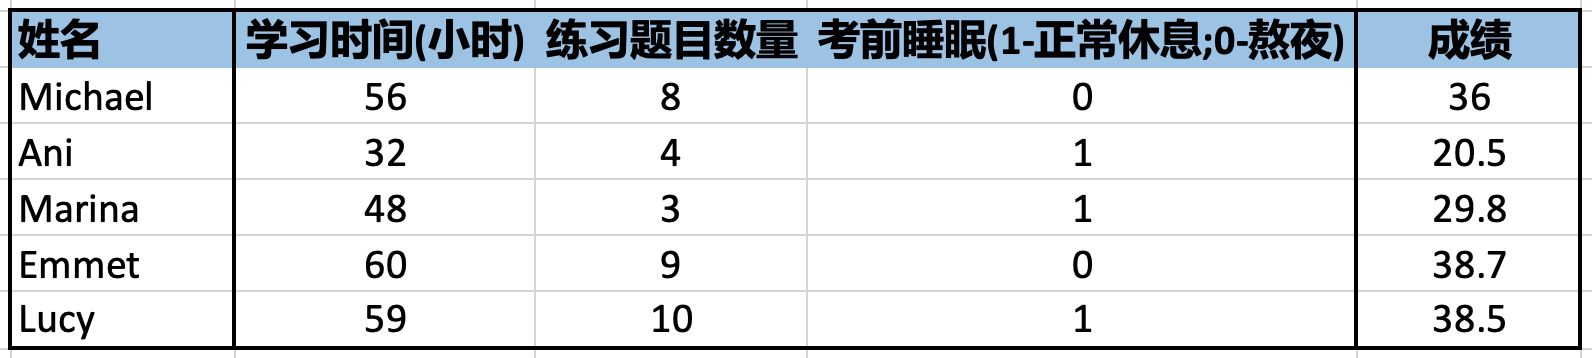
\includegraphics[width=0.8\textwidth]{fig/C1C2grade}
	\caption{学生学习状态和成绩统计}
\end{figure}

假设我们现在想调查,学习时间、练习题目数据和考前睡眠对成绩的影响,那么我们可以把上面的问题抽象为一个数学问题,表现为下面的表格。
\begin{figure}[H]
	\centering
	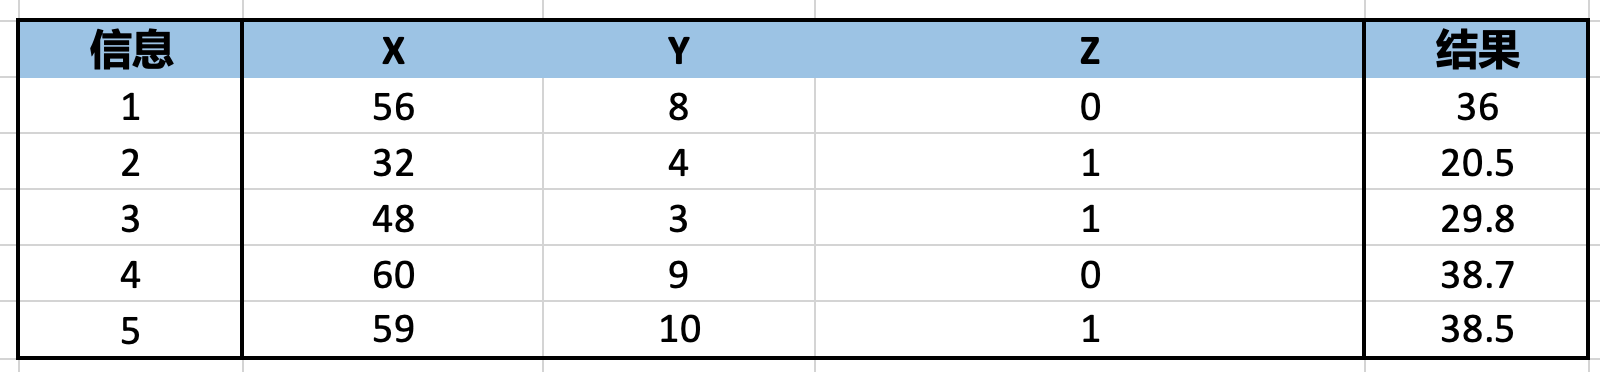
\includegraphics[width=0.8\textwidth]{fig/C1C2gradeMath}
	\caption{具体问题抽象数学化}
\end{figure}
那么通过解方程的方式,我们可以得出:
\begin{itemize}
	\item $x = 0.6$, 即学习时间对成绩的影响比重约为60\%;
	\item $y = 0.3$, 即练习题目的数量对成绩的影响比重约30\%;
	\item $z= 0.1$, 即考前睡眠对成绩的影响比重约10\%。
\end{itemize}

\begin{fullmodel}
现实生活中有很多问题,都可以上述方法来进行解答。比如下面这个数据阵,是从一个$414\times7$的数据阵中截取的一部分,该数据阵描述的是台北市房屋价格与其位置和周边环境的关系(数据来源:Prof. I-Cheng Yeh)。
\begin{figure}[H]
	\centering
	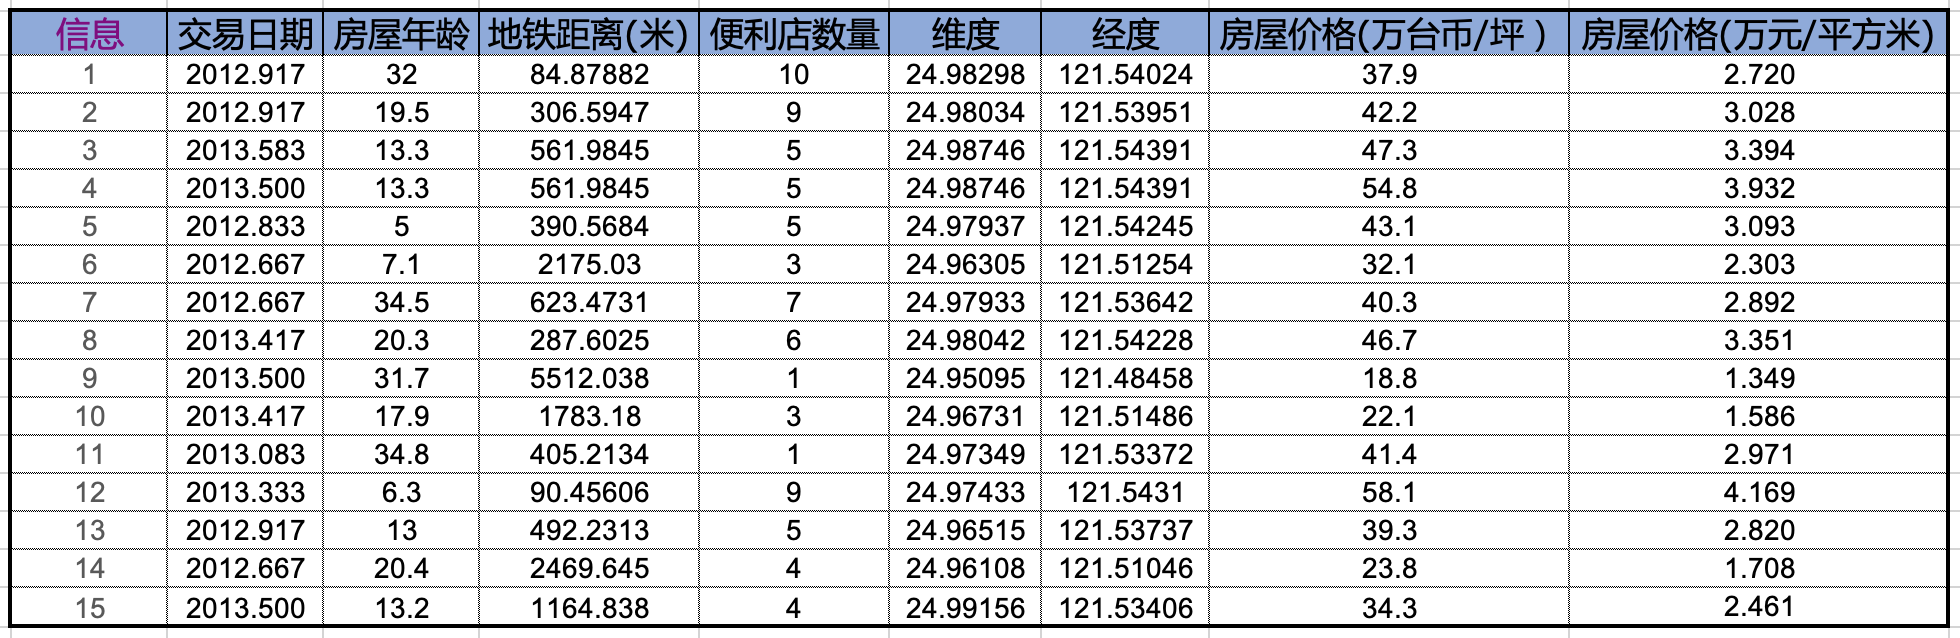
\includegraphics[width=0.86\textwidth]{fig/C1C2RealEst}
	\caption{台北市房屋价格与周边环境关系数据阵}
\end{figure}

在我们解方程之前,我们先将部分数据进行可视化,从而可以更直观的观察这些影响因子与房屋价格之间的关系。
\begin{figure}[H]
	\centering
	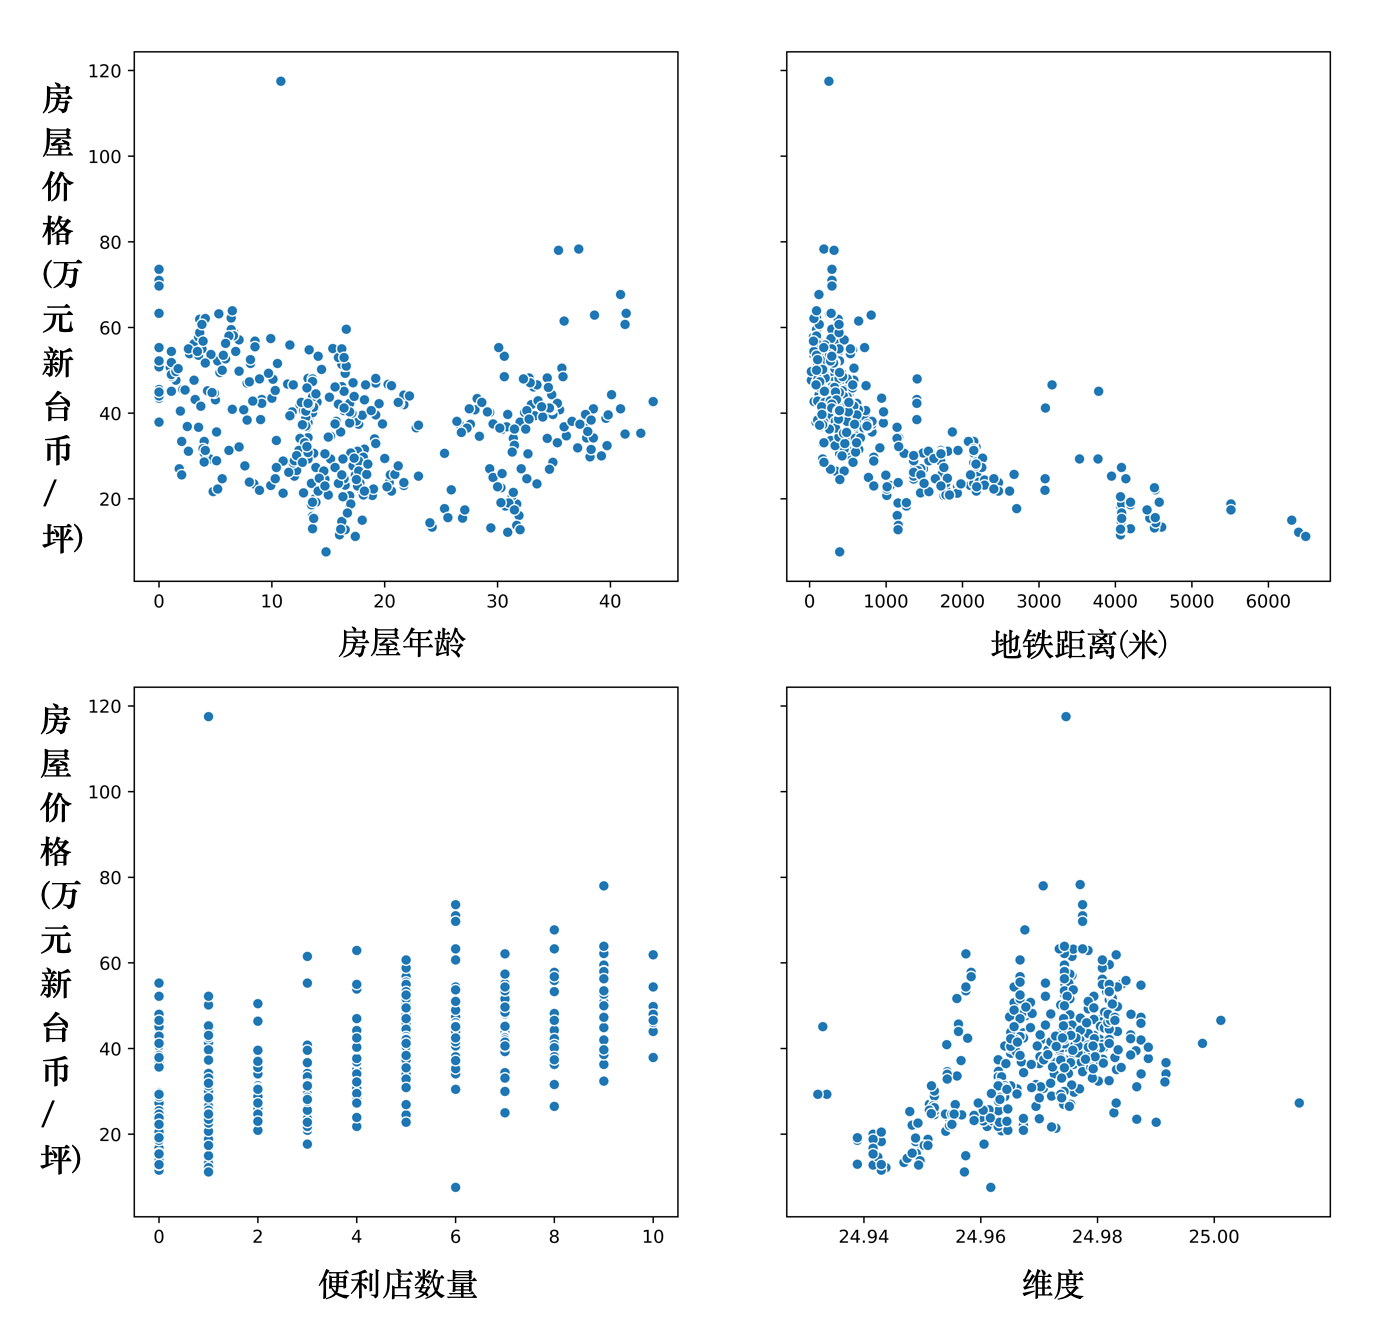
\includegraphics[width=0.7\textwidth]{fig/C1C2TbRealEst}
	\caption{台北市房屋价格与周边环境关系的可视化}
\end{figure}
\end{fullmodel}

下面,我们仍然利用`解方程'的思路去调查这些影响因子对台北市房价的影响比重。简单的计算可以得出:
\begin{itemize}
	\item 房屋年龄影响因子数为$-0.269$, 可以理解为房屋年龄每增加一年,房价下降$0.269$万新台币每坪;
	\item 地铁距离的影响因子数为$4.26$, 可以理解为地铁距离每增加1000米房价下降约$4.26$万新台币每坪;
	\item 便利店数量:1.163
	\item 维度: 2.38 (台北人买北不买南)
	\item 经度: -7.8 (买西不买东)
\end{itemize}

\begin{fullmodel}
	\begin{tcolorbox}[title={从线性回归到机器学习}]
		在上面的几个例子中,我们都用到了`解方程'的思路。实际上,在统计学中,该方法被叫作\textbf{线性回归}, 即假定不同影响因子与其所作用的结果之间存在线性的关系,比如:
		\begin{align*}
			36x + 18y + 0.3 z + \cdots -3w - 0.5 r = \text{结果} 
		\end{align*}
		假定这些影响因子与其所作用的结果存在线性关系后,我们就可以利用`解方程'的思路在求解这些影响因子, 限定条件为:信息量大于影响因子(独立方程个数大于未知数)。
		
		但是在现实生活中,很多规律或者事物之间的逻辑关系,并不是简单得线性关系。另外很多规律或者事物之间的逻辑关系,并不能通过数学公式或者模型来表达。因此,这就需要我们借助更加复杂的机器学习模型,和神经网络模型。
		
		所以我们需要机器学习的原因为:
		\begin{itemize}
			\item 所研究的问题中存在的规律非线性,即不能简单的概括为类似于$36x + 18y + 0.3 z + \cdots -3w - 0.5 r = \text{结果} $这样的公式;
			\item 所研究的问题中存在的规律不仅非线性,而且不能用简单得数学公式去概括,因为
			\begin{itemize}
			\item 这些公式要么非常复杂,不可以通过编程实现
			\item 或者根本就不存在统一的数学公式组或公式群去描述这些规律
			\end{itemize}
		\end{itemize}
	\end{tcolorbox}
\end{fullmodel}

那么了解了何谓机器学习之后,我们将会:
\begin{itemize}
	\item 在第二章,介绍如何通过机器学习解决所研究的问题存在的规律非线性\mn{线性指的是只存在相乘和相加关系,因为乘法实际也是加法,比如$5\times3 = 5+5+5$,所以只有相乘和相加时,我们可以把所有的因素`排成一条线'累加。}。
	\item 在第三章和第四章,介绍所研究的问题根本就不存在统一的公式时,神经网络模型(深度学习)如何应对。
\end{itemize}

\subsubsection{机器学习解决问题的方法}

因为很多问题不能通过简单得解方程(线性模型)方式来解决,或者很多问题背后的规律根本就不存在`简明'得数学公式或者数学公式及其复杂不能被编程实现,那么就需要我们探索新的解决问题的思路。

在本章的介绍中,我们在图1.1中展示了,机器学习解决问题的方法是:输入结果和数据,然后通过相关模型来学习背后的规律或者范式。那么机器学习和更加复杂的神经网络模型是如何来学习这些规律的呢?如果用一句话来概括的话,我们可以说:\textbf{机器学习(包括神经网络模型)是通过有结果导向的数据来学习数据背后的规律的}。具体的流程可以概括为下面的流程图。
\begin{figure}[H]
	\centering
	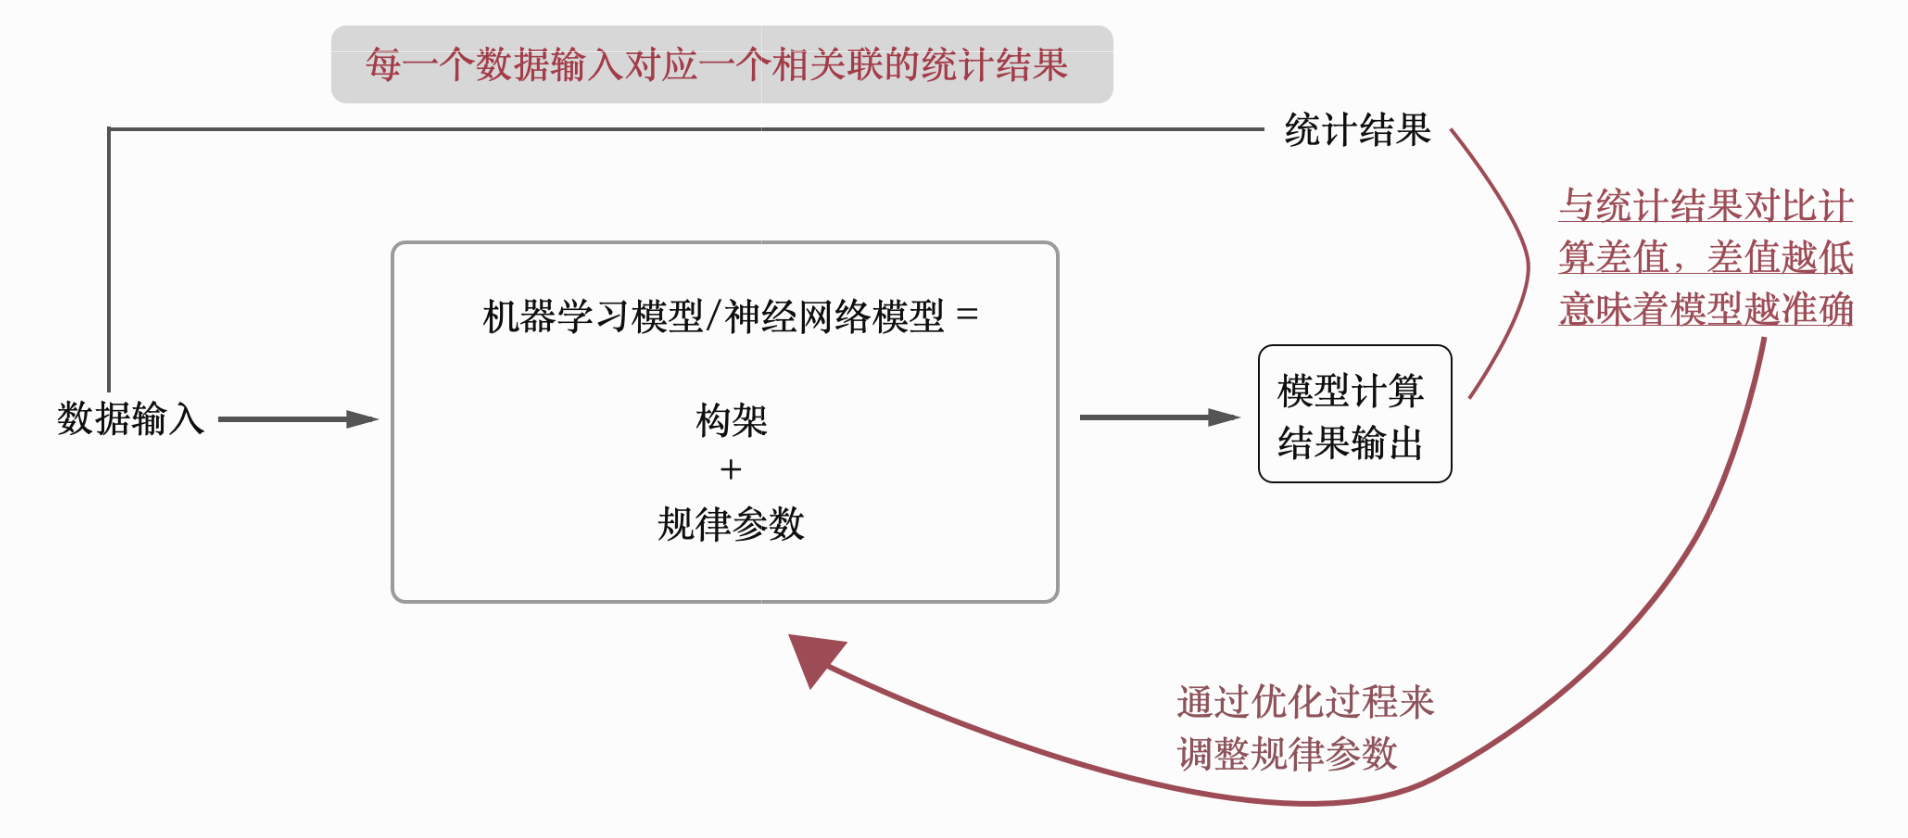
\includegraphics[width=0.9\textwidth]{fig/C1C2MLMechanism}
	\caption{机器学习框架流程图}
\end{figure}

我们再重温下机器学习的定义:
\begin{remark}
\textbf{机器学习}指的是计算机根据一定的算法在有数据的支持下完成某一规律的学习,并且对所学习到的规律进行自动化调整。	
\end{remark}

在定义中,
\begin{itemize}
	\item 算法即包括\textit{具体的构架},也包括优化过程中的算法;
	\item 有数据支持意味着,除了有初始数据输入之外,还得有相对应的结果来支持模型进行结果衡量;
	\item 对某一规律的学习,指的是对\textit{规律参数}的计算
\end{itemize}

\begin{fullmodel}
	\begin{tcolorbox}[title=冰冻三尺非一日之寒]
		在大体了解了机器学习解决问题的方法后,我们需要通过学习不同的模型和进行大量练习来深入理解其框架流程。因此,在第一章中我们只是希望同学们有个大的概念,后续过程中再`一砖一瓦'来丰富这个框架和流程。希望同学们在学习后面不同的模型和具体的应用时,可以时常回到第一章来进一步领会图1.7的框架和概念。
	\end{tcolorbox}
\end{fullmodel}

\subsubsection{人工智能思维原素}

在本章的最后一个小节中,我们特别提醒同学们,在以后的学习过程中,注意积累以下的素养。这些素养可以说是人工智能思维的基本原素,他们包括:
\begin{itemize}
	\item 数据思维,比如每次你做练习时,思考下,这个数据是什么结构,是如何标注的,维数是怎么样的,等等;
	\item 计算机思维,比如每次接触不同模型时,思考计算机是如何程序化计算得等等;
	\item 机器学习思维,比如思考整个机器学习模型时如何构建和训练,以及预测的。
\end{itemize}

以下是本章中使用到的Python代码,供有兴趣的同学参考。注意其中涉及\texttt{TensorFlow}部分的代码不要过多得去研究。在高中阶段我们暂时不会讲解。
\begin{python}
# Chapter 1 C1 C2 Code
# 第一章
# @ Michael


import os
import numpy as np
import pandas as pd
import matplotlib.pyplot as plt
import seaborn as sns
from sklearn.linear_model import LinearRegression
from sklearn import preprocessing
import tensorflow as tf
from tensorflow import keras


# set the working direction
os.getcwd()
os.chdir('/Users/Michael/Documents/MDLforBeginners/Chapter1/Code')

# define a simple function(定义一个方程)
def fx(x):
    """
    A simple function for calcuating:
        f(x) = x^2 + 2x - 3
    Input: x - 1 by n vector
    Output: return f(x) 1 by n vector
    """

    y = np.power(x, 2) + 2 * x - 3

    return y


# Test the function(测试方程)
x = np.array(range(1, 10))
print(fx(x))


# A simple nueral network model for learning the function fx
# Reference: Laurence Moroney
def Learn_model(y_new):
    xs = np.array([1.0, 2.0, 3.0, 4.0, 5.0, 6.0, 7.0, 8.0], dtype=float)
    ys = np.array([0.0, 5.0, 12.0, 21.0, 32.0, 45.0, 60.0, 77.0], dtype=float)
    model = tf.keras.Sequential([keras.layers.Dense(units=1, input_shape=[1])])
    model.compile(optimizer='sgd', loss='mean_squared_error')
    model.fit(xs, ys, epochs=800)
    return model.predict(y_new)[0]


prediction = Learn_model([9.0])
print(prediction)


def c1c2fun1(x):
    """
    解方程 56x + 8y = 36
    输入: x
    输出: y
    """
    y = (36-56*x)/8

    return y


print(c1c2fun1(np.array(range(0, 8))))
# [ 4.5 -2.5  -9.5 -16.5 -23.5 -30.5 -37.5 -44.5]


# Linear regression for predicting house price
# read the dataset
tb_real_estate = pd.read_excel('Real estate valuation data set.xlsx')
tb_real_estate.shape
tb_real_estate.head()
tb_real_estate.columns
# Index(['No', 'X1 transaction date', 'X2 house age',
#        'X3 distance to the nearest MRT station',
#        'X4 number of convenience stores', 'X5 latitude', 'X6 longitude',
#        'Y house price of unit area'],
#       dtype='object')

# Data visualization
fig, axes = plt.subplots(2, 2, figsize=(12, 12), sharey=True)  # share y
sns.scatterplot(x=tb_real_estate['X2 house age'],
                y=tb_real_estate.iloc[:, 7],
                ax=axes[0, 0])
sns.scatterplot(x=tb_real_estate.iloc[:, 3],
                y=tb_real_estate.iloc[:, 7], ax=axes[0, 1])
sns.scatterplot(x=tb_real_estate.iloc[:, 4],
                y=tb_real_estate.iloc[:, 7], ax=axes[1, 0])
sns.scatterplot(x=tb_real_estate.iloc[:, 5],
                y=tb_real_estate.iloc[:, 7], ax=axes[1, 1])
fig.savefig('taibeiRealEst.png', dpi=800, bbox_inches='tight')

# run regression
tb_X = tb_real_estate.iloc[:, 2:7]
tb_Y = tb_real_estate.iloc[:, 7:8]

tb_reg = LinearRegression()
tb_reg.fit(tb_X, tb_Y)
tb_reg.coef_
# array([[-2.68916833e-01, -4.25908898e-03,  1.16302048e+00,
#          2.37767191e+02, -7.80545273e+00]])
tb_reg.intercept_

# notice that it does not make sense for normalizing the distance!
tb_x_norm = preprocessing.normalize(tb_X)
tb_norm_reg = LinearRegression()
tb_norm_reg.fit(tb_x_norm, tb_Y)
tb_norm_reg.coef_
# array([[-6.71038947e+01,  7.82866997e+01,  1.79603302e+02,
#          8.48265938e+04, -1.73503097e+04]])
# the second coefficient should be negative
#
\end{python}

\subsection{课后练习C3}

本章的课后练习着重让同学们去探索机器学习在不同场景中的应用,不涉及具体的计算。

\begin{question}{C3-Q1}
	刘清宇同学很喜欢听音乐,他的手机里存放了大约有200首他多年筛选下来的歌曲。但是他觉得还是不够听,可是每次想要去搜寻符合他的审美乐趣的歌曲时都很花费时间,请问你可以想一个方法来帮助刘清宇同学来推荐符合他的审美乐趣的歌曲吗?
\end{question}


\begin{question}{C3-Q2}
	请同学们到网络上搜索一个机器学习的应用场景,然而思考它是如何按照图1.7中的框架流程来结局在你选在的应用场景中解决具体问题的。
\end{question}


\noindent
\textcolor{purple}{疑难解答}:如果有相关疑问,请扫描下面的二维码,将你的问题输入,老师会尽快答疑解惑:$\heartsuit$。 \begin{marginfigure}
	\centering
	
\includegraphics[width=\textwidth]{fig/C1C3qrcode}
\end{marginfigure}



\newpage
\setcounter{section}{2}
\part*{第二章: 简单分类-察异辨花}

从这一章开始,我们就正式进入了机器学习相关模型的介绍。这一章的主题是`简单分类',我们之所以选择这一主题作为机器学习模型的最初介绍,是因为在人工智能领域,有超过一半的任务是处理分类问题,比如信用卡违约识别是从消费人群中分别出哪些消费者更可能会违约,再比如较为复杂的人脸识别就是在千千万万个照片中将不同的人脸进行分类。

本章节中我们会重点学习两个模型:
\begin{enumerate}
	\item 简单的线性分类(感知器分类)
	\item 支持向量机\mn{Support Vector Machines}分类(可以进行非线性分类)
\end{enumerate}

按照惯例,本章的学习仍然有三部分组成:课前预习,课堂讲义,和课后练习。在课前预习中,我们将会讨论\textit{什么是分类,在什么情况下可以分类};在课堂讲义中,我们会在理解了分类的意涵后,来定义\textit{测量和优化},明白了测量和优化之后,我们便可以比较好得掌握简单的线性分类模型和支持向量模型。


\subsection{课前预习C1}

此次课前预习重点强化同学们对分类的理解,课前预习照旧包括两个部分:
\begin{itemize}
	\item 生活引导题: 思考你是如何分类的
	\item 简单的数学练习题
\end{itemize}


\noindent
\textit{第一部分: 生活引导题}

从生活中找一个分类的例子,然后描述下你是如何分类的(不超过60字),描述必须包含下面三个部分:
\begin{itemize}
	\item 分类的主体对象是什么?(比如,汽车,花草,等等)
	\item 分类的依据和标准是什么?
	\item 分类后如何衡量分类得好坏?
\end{itemize}


\noindent
\textit{第二部分: 简单的数学演练}

\begin{question}{C1-Q1}
	下面有一个数组$A$:
	\begin{align*}
		A  = [1, 3, 2, 5, 4, 7, 9, 11,  10, 16]
	\end{align*}
	你是否可以设计一个方程来将数组$A$中的奇数和偶数进行分类。如果有兴趣,你也可以尝试写一个Python小程序来完成该任务。
\end{question}


\begin{question}{C1-Q2}
	下面表格是我们从安德森鸢尾花卉数据集(Anderson's Iris data set)截取的一部分数据。
	\begin{table}[H]
		\centering
		\begin{tabular}{lccc}
		\hline 
			属种 & 代码 &花瓣长度 & 花瓣宽度 \\
			\hline 
			山鸢尾 & s1 & 1.4 & 0.2 \\
			山鸢尾 & s2 & 1.7 & 0.4 \\
			变色鸢尾 & ve1 & 3.9  & 1.4 \\
			变色鸢尾 & ve2& 4.9 & 1.5 \\
			维吉尼亚鸢尾 & vig1 & 6.9 & 2.3  \\
			维吉尼亚鸢尾 & vig2 & 6.1 & 1.9 \\
			\hline  
		\end{tabular}
	\end{table}
	下面的坐标中$X$轴代表花瓣长度,$Y$轴代表花瓣宽度,请将以上六个花朵定位到坐标系中去(用相应代码代表).
	\begin{figure}[H]
		\centering
		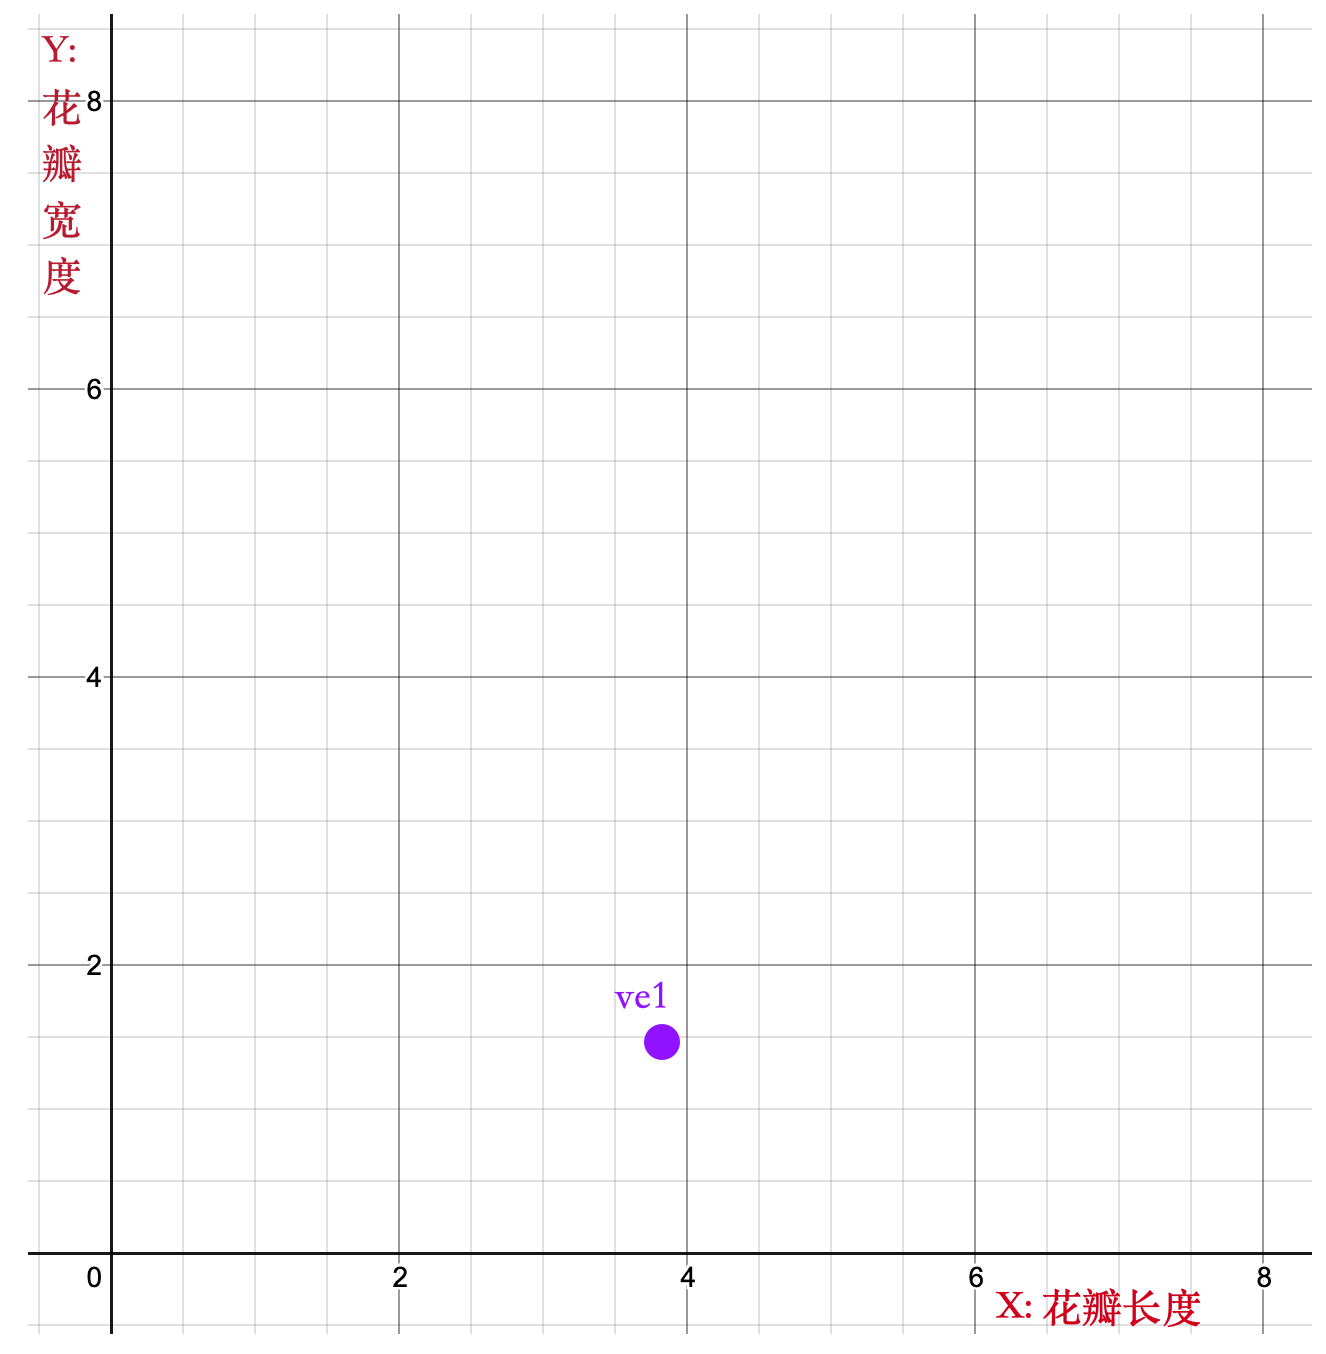
\includegraphics[width=0.6\textwidth]{fig/C2C1coord}
	\end{figure}
\end{question}

\begin{question}{C1-Q3}
	在生活中,我们经常需要用不同的数据来帮助我们记录一定的信息。比如下面这个数据阵中包含的就是不同葡萄酒的相关信息。
		\begin{table}[H]
		\centering
		\begin{tabular}{lcccc}
		\hline 
			葡萄酒 & 代码 &酒精度 & 苹果酸 & 颜色强度(1-10) \\
			\hline 
			品种1 & 0 & 14.23 & 1.71 & 5.64 \\
			品种1 & 0 & 13.20 & 1.78 & 4.38  \\
			品种2 & 1 & 12.17  & 1.45 & 2.95 \\
			品种2 & 1& 12.37 & 1.21 & 4.60  \\
			品种3 & 2 & 13.71 & 5.65 & 7.7   \\
			品种3 & 2 & 13.17 & 2.59 & 9.3 \\
			\hline  
		\end{tabular}
	\end{table}
\end{question}

按照同样的道理,我们也可以把这些普通酒的种类在三维图中定位,如果$X$代表酒精度,$Y$代表苹果酸,$Z$代表颜色强度,那么下图就是不同葡萄酒在这三个数据描述下的定位。
	\begin{figure}[H]
		\centering
		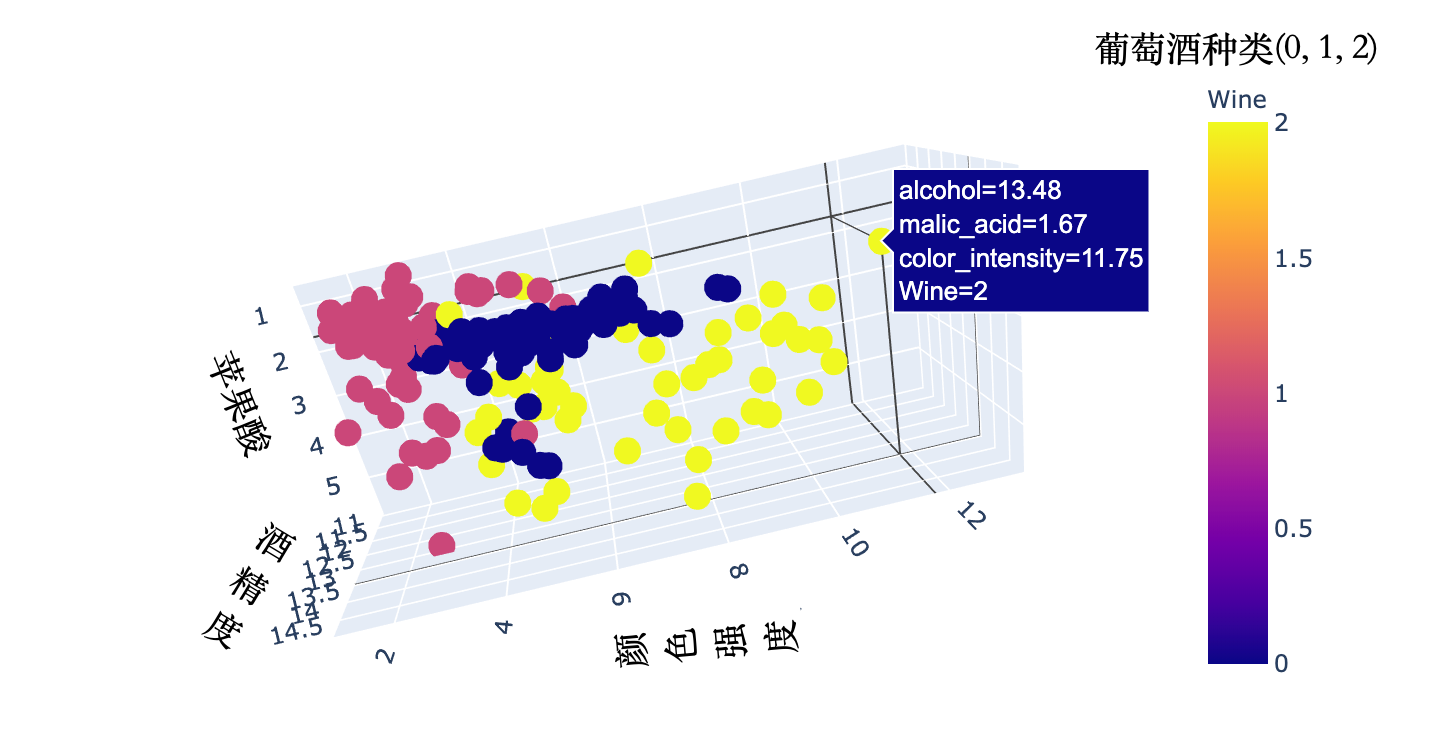
\includegraphics[width=0.69\textwidth]{fig/C2C1wine}
	\end{figure}

\begin{tcolorbox}[title=为什么要将数据可视化]
		我们通过几个预习的题目,是想通过数据的可视化让同学们有对分类有更直观的认识。也就是说,尽管不同种类的物体可能在某些数据维度上有所交叉,但是只有某一个维度有明显的差异,那么表现成\textbf{集群}后,其可分类的可能性就会大大提升。另外,需要提醒同学们的是,当对一个物体的描述超过3个时,就很难再进行可视化演示,因为我们只能进行三维构图,超出三维的同学们只能借助三维的图片在进一步想象。
\end{tcolorbox}

\begin{question}{C1-Q4}
		我们有下面两个表格,很明显如果只给你第一个表格的话,你是无法进行分类的。但是增加了数据描述后,我们发现,分类就变得很容易。
\end{question}
\begin{table}[H]
	\centering
		\begin{tabular}{ll}
\begin{tabular}{ccc}
车型 & 动力 & 座位数  \\
\cline{1-3}
A & 169 & 4 \\
A & 169 & 4 \\
B & 169 & 4\\
B &  169 & 4  \\
\hline 
\end{tabular}
&
\begin{tabular}{cccc}
车型 & 动力 & 座位数 & 油耗 \\
\cline{1-4}
A' & 169 & 4 & 6\\
A' & 169 & 4 & 6 \\
B' & 169 & 4 & 9 \\
B' &  169 & 4 & 9 \\
\hline 
\end{tabular}
\end{tabular}
\end{table}
现在如果我们把相关的数据统计在向量中表达我们可以发现:
\begin{align*}
	A - B & = [169, 4] - [169, 4] = [0, 0]  \\
	A' - B' & = [169, 4, 6] - [169, 4, 9] = [0, 0, -3] 
\end{align*}


\begin{tcolorbox}[title={向量和矩阵本身就是一种可视化}]
		通过这个例子我们可以发现,当我们对一个物体的描述大于3时,虽然不能进行可视化来进行快速分类,但是我们可以通过向量运算来进行分类,比如下面这三个向量。
\end{tcolorbox}

\begin{align*}
	A& = [0, 1, 9, 17, 100] \\
	B & = [0, 2, 9, 17, 100] \\
	C & = [0, 1, 9, 10, 56] 
\end{align*}

\begin{question}{C1-Q5 解方程}
	我们再做几个个解方程题目, 求解$x, y$
	\begin{align*}
		2x + 3y & =1 \\
		x + y & = -1 
	\end{align*}
	求解$x, y, z$
	\begin{align*}
	& 56x + 8 y = 36 \\
	& 32 x + 4 y + z = 20.5 \\
	& 48 x + 3y + z = 29.8 
\end{align*}
\end{question}

\begin{fullmodel}
	上面的预习题目C1-Q5中,我们可以把$x, y, z$的方程组进行下列转换:
	\begin{align*}
		56x + 8y -35 & = 36 - 35  \ \ \Rightarrow 56x + 8y -35 = 1\\
		32x + 4y + z - 21.5 & = 20.5 - 21.5 \ \ \Rightarrow 32x + 4y + z - 21.5  = -1 \\
		48x + 3y + z - 30.8 & = 29.8 - 30.8  \ \ \Rightarrow 48x + 3y + z - 30.8 = -1  
	\end{align*}
	从而得到下列方程组
	\begin{align*}
		56x + 8y -35 & = 1\\
		32x + 4y + z - 21.5 &  = -1 \\
48x + 3y + z - 30.8 & = -1 
	\end{align*}
\end{fullmodel}


\subsection{课堂讲义C2}

本章节的课堂讲义较为重要\mn{本章可以说是全书的重中之重,如果本章的学习同学们能够领会和进行实验操作,那么后面的章节都会`不在话下’。},希望同学们认真阅读。我们会在本章的课堂讲义中,逐步介绍以下的知识点:
\begin{itemize}
	\item 什么是分类
	\item 什么是线性分类
	\item 什么是非线性分类(引入支持向量机)
\end{itemize}

\begin{fullmodel}
	\begin{tcolorbox}[title=没有你学不会的,只有老师教不懂的。]
		有同学在读本章的教材时,会觉得有些数学公式较为复杂,可能会觉得自己不适合学习人工智能。这里我想特别给同学们一些温馨提示:
		\begin{enumerate}
			\item 只要你会计算$1+2=3$,并且会解一元二次方程组,那么老师可以保证你可以理解全部内容;
			\item 在计算机和人工智能的模型辅助下,几何任何计算都可以由电脑完成,所以同学们要着重对\textbf{相关概念进行深层次了解},从而可以调用电脑代码来执行你的想法。
			\item 想象力,以及对事物的抽象能力,将是老师对你们的训练重点,所以不要怀疑自己的数学认知,或者对数学有抵触。
			\item 当然你如果对$1+2=3$这样的问题也很费解的话,老师会鼓励你在其它方面,比如绘画、美食等等行业进行自我开显。
		\end{enumerate}
	\end{tcolorbox}
\end{fullmodel}


\subsubsection{什么是分类}

\begin{definition}
	分类指的是根据事物不同的属性,对某个或一些物体进行划分的过程。在没有任何属性的情况下,我们不能进行分类。在有属性的情况下,我们可以依据属性,进行分类,比如黑猫和白猫。
\end{definition}

\begin{remark}
从哲学的角度上讲,存在的便是有属性的在。绝对的存在(即无属性的纯存在)在中文哲学的概念里指的是`道’\mn{老子里有一句名言: 道生一,一生二,三生万物。},在西方哲学里指的是`上帝'。黑格尔有一句名言:绝对得有即是绝对得无。	
\end{remark}

\begin{tcolorbox}[title=分类等同于属性界定]
	一旦明白了什么是分类之后,我们就可以说: \textit{分类就等同于对事物属性的界定和划分}。比如,下面的例子:
	\begin{itemize}
		\item 根据发型区分男人和女人
		\item 根据哺乳方式区分哺乳动物和非哺乳动物
	\end{itemize}
\end{tcolorbox}

因为事物的属性可以是很繁杂的,比如自然界中光是树木的科目分类就达到几万种(如果考虑不同植被的话,这个科目的量级会进一步上升)\mn{有兴趣的同学可以去央视科教频道看下2007年国家最高科学技术奖吴征镒的采访,以吴先生提出的被子植物八纲系统,进行分析不仅有助于认识中国被子植物的全貌,也有助于理解世界植物区系的形成和发展}。所以我们在对这些属性进行界定时,最简单有效的方式就是对其数字化(或者说有数字去测量和统计),比如下面这个案例。
\begin{table}[H]
		\centering
		\begin{tabular}{lccc}
		\hline 
			属种 & 代码 &花瓣长度 & 花瓣宽度 \\
			\hline 
			山鸢尾 & s1 & 1.4 & 0.2 \\
			山鸢尾 & s2 & 1.7 & 0.4 \\
			变色鸢尾 & ve1 & 3.9  & 1.4 \\
			变色鸢尾 & ve2& 4.9 & 1.5 \\
			维吉尼亚鸢尾 & vig1 & 6.9 & 2.3  \\
			维吉尼亚鸢尾 & vig2 & 6.1 & 1.9 \\
			\hline  
		\end{tabular}
\end{table}

\begin{lemma}
	当两个或多个事物的属性不同时,我们将会根据他们不同的属性进行分类。因此一类事物,即是有一连串属性所界定的。比如,马 = 有四肢+食草类动物 + 眼睛处于两侧+等等等。如果两个或多个事物的属性没有差异,我们要么在现有信息下不能分类,要么需要寻找更多的信息进行分类。
\end{lemma}

\begin{example}
下面我们看一个具体的案例,下图中分别显示了不同性别的身高(height)和体重(weight)	。
\begin{figure}[H]
	\centering
	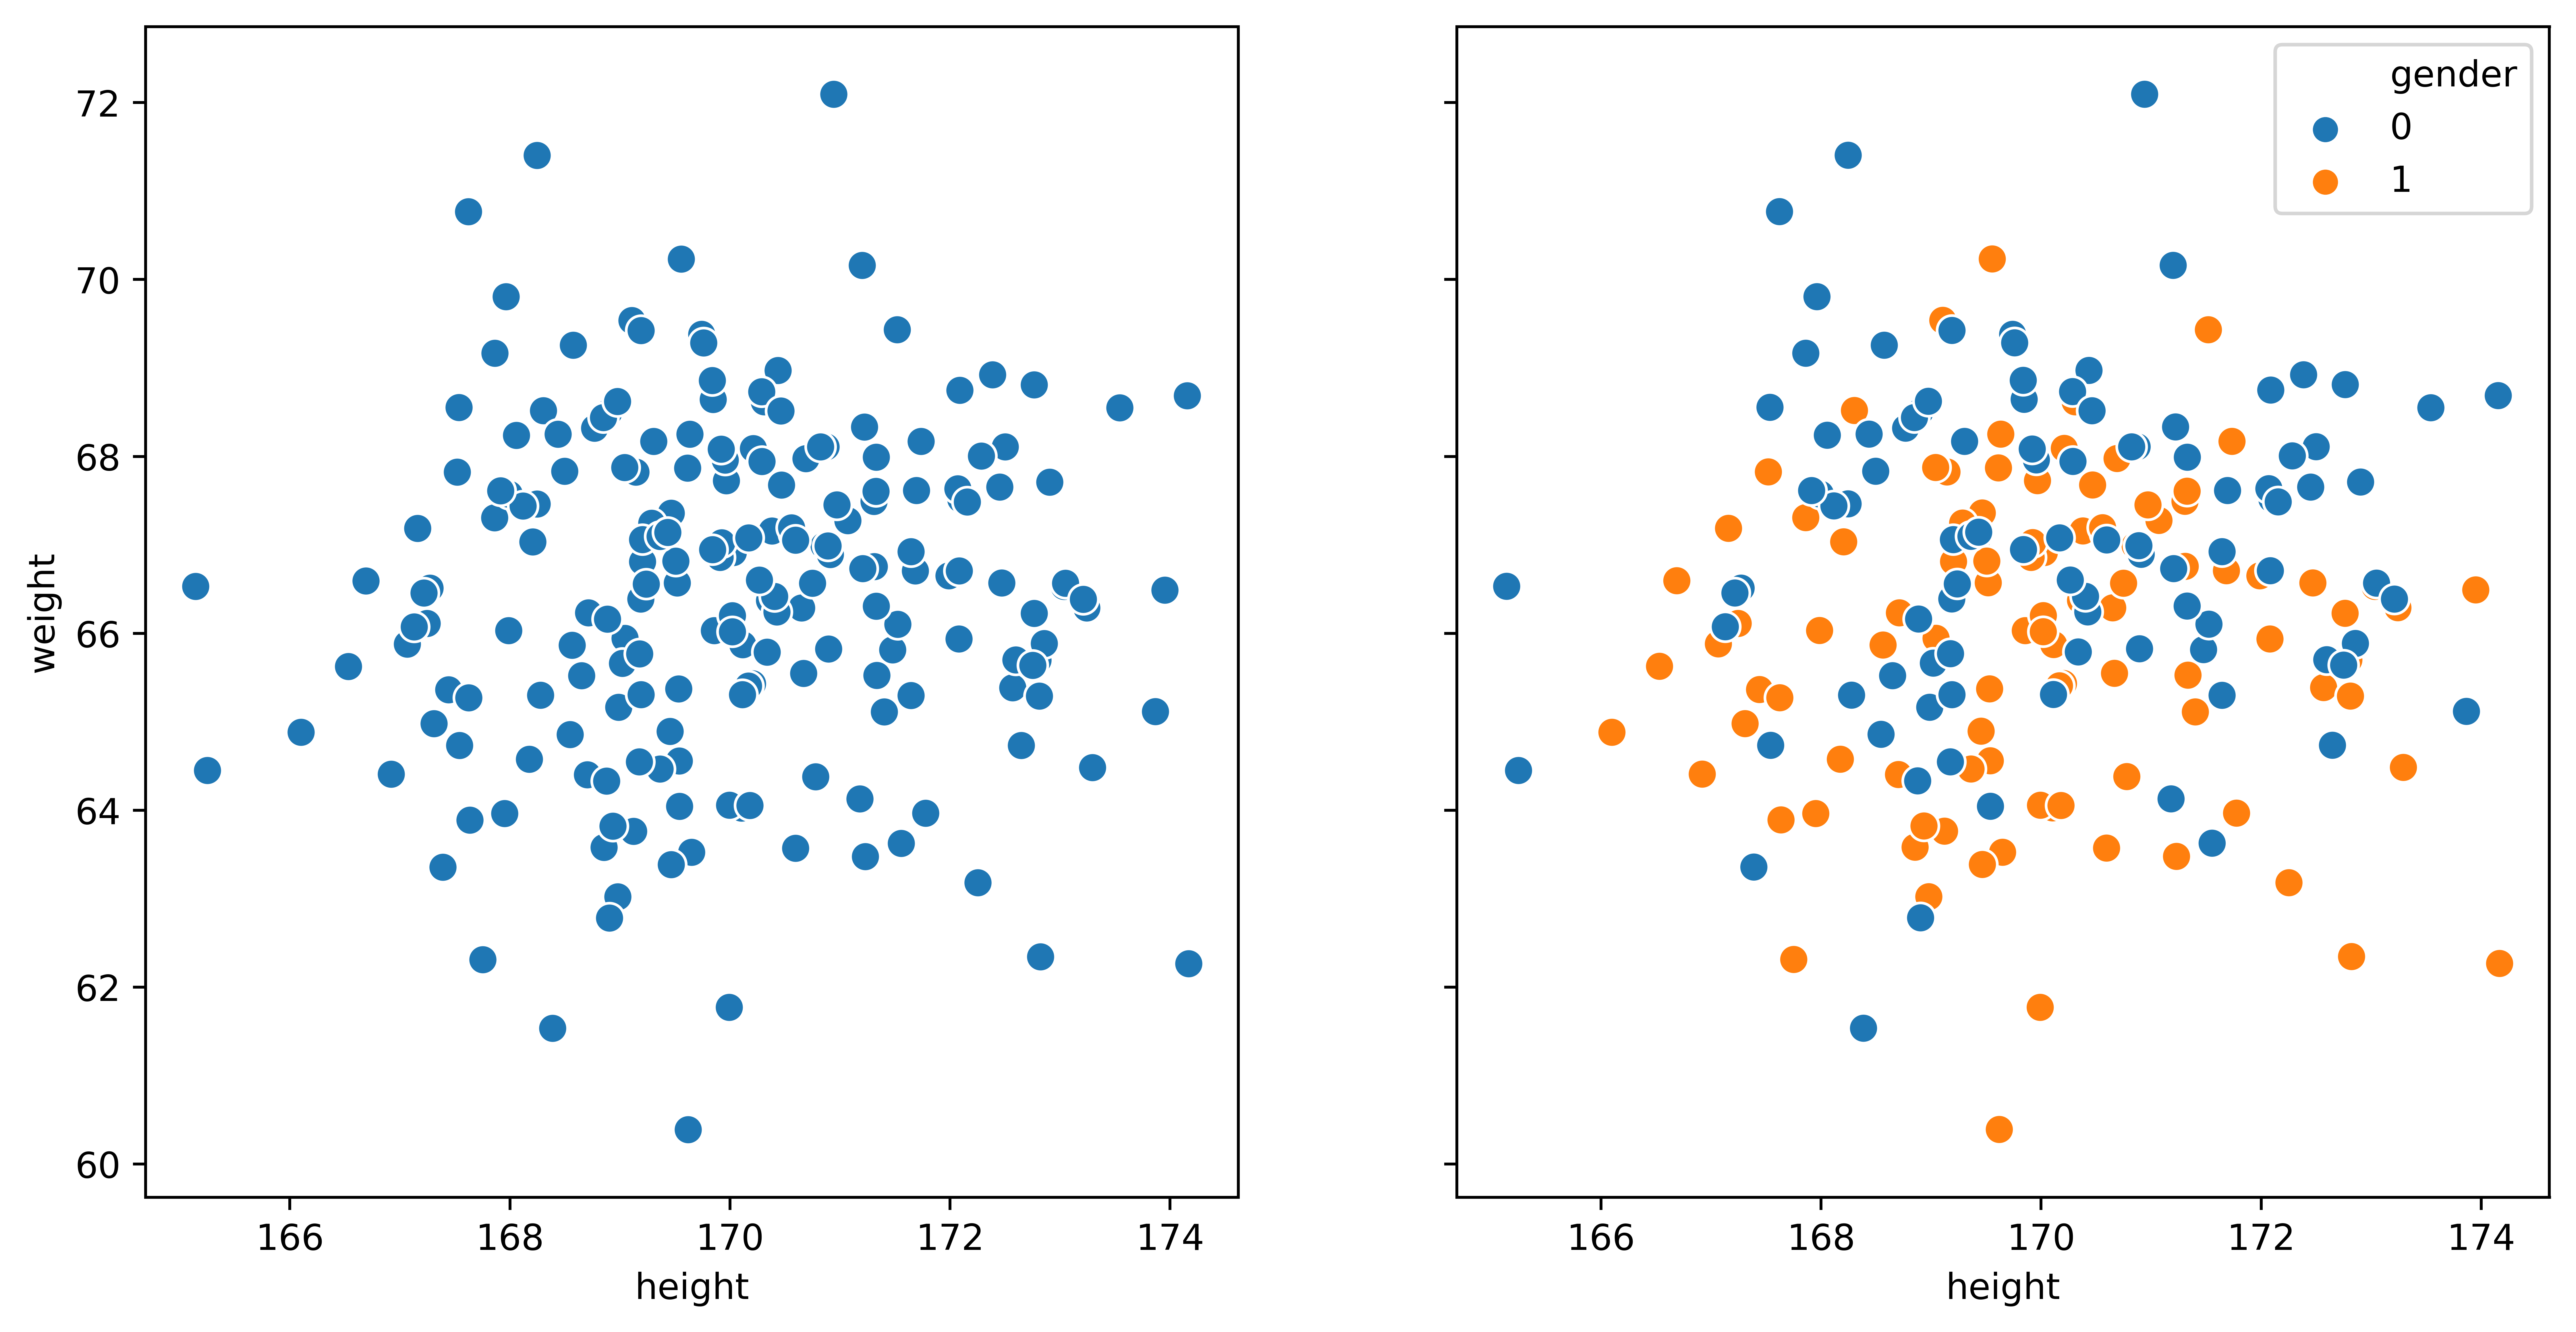
\includegraphics[width=0.8\textwidth]{fig/BMI}
\end{figure}
\end{example}


在上面的这个例子中,如果我只给你左边的数据或者图片,很显然你是无法进行分类的。或者你只能如此分类:
\begin{itemize}
	\item 分类一: 身高小于170cm的人
	\item 分类二: 体重大于70公斤的人
\end{itemize}
但是仅仅凭这些信息,你是无法分辨这些人的性别的。如果我们将这些数据进行3D可视化的话,那么分类就会变得更容易。




































\newpage
\part*{第三章:神经网络模型初探}

\marginnote{\begin{tcolorbox}[colframe=gray]《大学》中语:知止而后有定,定而后能静,静而后能安,安而后能虑,虑而后能得。物有本末,事有终始。知所先后,则近道矣。\end{tcolorbox}}

亲爱的同学们,从这一章开始我们将会接触目前比较流行的人工智能模型-神经网络模型。相较前一章节,本章难度有所提升,而且模型背后的相关概念更加抽象。如果你已经开始阅读第三章节的内容,或许你会觉得\textit{`不知所云'}或者\textit{`无从下手'}。 对于任何一个初学者来说,这都是很正常的经历,希望你们不要气馁,更不要怀疑自己。此时此刻,希望同学们仍然要怀着探索的心态去进入这一章节的学习。

我们将会在接下来的三周里沉浸在神经网络模型中,如果同学们紧跟老师的节奏,按照要求完成\textbf{课前预习,课上笔记,及课后练习}这三个环节,我可以向你们保证,三周之后你们(每一位同学)完全可以:
\begin{itemize}
	\item 理解为什么人工智能在神经网络\sn{Neural Network}出现后具有了广泛得应用价值;
	\item 掌握神经网络的本质所在,并且了解模型背后的思想精髓所在;
	\item 能够用Python透过向量\sn{Vector}和矩阵\sn{Matrix}进行编写20行左右的小程序,从而以此去理解神经网络的模型设计逻辑;
	\item 能够使用Python中人工智能学习平台,如TensorFlow来进行神经网络的训练和调试,从而可以独立自主得对大量的图片数据进行分析。
\end{itemize}

%\marginnote{\begin{tcolorbox}[colframe=gray]jh\end{tcolorbox}}


\setcounter{section}{3}
\setcounter{subsection}{0}
\subsection{课前预习C1}

本次C1依然两部分组成:
\begin{enumerate}
	\item 读网络文章, 看网络视频;
	\item 根据指示完成小习题,并且准备在课上使用。
\end{enumerate}

\noindent
\textit{第一部分: 神经网络追本溯源}

人们对人工智能的研究热情由来已久,其中神经网络模型的主要研究兴起于上世纪八十年代。众多研究者中,领军人物包括但不限于:Geoffrey Hinton\mn{杰弗里·辛顿},  Yoshua Bengio and Yann LeCun。他们三位因此也被称为人工智能三教父\mn{Godfathers of AI (Godfathers of Deep Learning)}。我们以Geoffrey Hinton的思路为切入点,来理解神经网络的发展过程和之所以蓬勃发展的深层次原因。

观看Geoffrey Hinton的采访视频,注意思考以下几个问题:
\begin{itemize}
	\item 观看前10分钟\mn{注意视频中配有机器自动加注的英文字母和中文翻译,因此存在一定纰漏,但是不影响整体理解.其中03:50处,他讲到`I think around early 1982...’,而不是`伊拉克发生了什么’。这说明机器和人类一样并不完美,`绝对'的物只在意念中存有!}
	\item 是什么触发了Geoffrey Hinton对人工智能的研究,最初的切入点是什么?
	\item Geoffrey Hinton 比较了英国和美国的学术环境,你从中有什么启发?
	\item Geoffrey Hinton 提到了心理学界和AI领域对\textit{知识}的理解,何谓知识?
	\item 视频连接:\url{https://www.bilibili.com/video/av69581590/}
\end{itemize}

\definecolor{steelteal}{RGB}{95, 124, 138}

\begin{fullmodel}
	\begin{tcolorbox}[title={哲学延伸},fonttitle=\large,colframe=medblue]
		   认识论是哲学研究范畴中比较重要的一枝,视频中Geoffrey提到`how concepts are relate to other concepts' (一个概念与其它概念的联系),这是目前有关知识的普遍共识。比如描述一朵花,需要高度,大小,颜色,等等一系列的概念堆积。而这些概念的关联就构成了我们的知识。\textbf{后面我们介绍深度学习模型时,你会接触到`卷积'和`池化'等概念}。这些新鲜的名字背后本质上是通过一个个数学模型来模拟概念关联和堆积,从而进行智能判断。深度神经学习本质上是对人的\textbf{生物仿生模拟},我们在调试模型时需要反向调整参数,这与我们实际生活中的学习如出一辙。比如,你第一次接触滚烫的热水时,会感到疼痛,接受到该信号后,下一次你会\textbf{试探性}得调整动作去接触热水,这就是人类反向调整的过程。
		   
		\setlength{\parindent}{5ex}
		Geoffrey能够想出神经学习模型除了与他自己兴趣广泛,对该问题长期关注之外,还与其在英国接受的教育传统有关。认识论的鼻祖可以追溯到笛卡尔(也就是发明XY坐标的那个法国人),但是第一次系统提出`所有的知识都是关联’的是英国哲学家休谟,休谟又启发了德国的大哲学家康德。人类历史上几次\textbf{颠覆}性的概念,如牛顿万有引力,达尔文进化论,休谟的认识论,亚当斯密的市场经济理论,图灵的计算边界论等都首先出自英国,是因为长期以来英国教育注重热爱自然,着重培养学生仔细观察记录和思考有关。同学们正值青春年华,不要泯灭了对自然和生命得热爱。以后人工智能可以帮助人类去完成更多机械化的任务,那么想象力就变得更加重要。
	\end{tcolorbox}
\end{fullmodel}

观看华为总裁任正非的采访视频,注意思考以下几个问题:
\begin{itemize}
	\item 观看视频中10:00 - 15:00分钟段
	\item 为什么任正非说人工智能是`计算机+统计学'?
	\item 为什么有一种论调称`数据就是未来的石油’?
	\item 视频连接:\url{https://m.sohu.com/a/290453977_652527/}
\end{itemize}

\begin{fullmodel}
	\begin{tcolorbox}[title={打破人工智能的迷思},fonttitle=\large,colframe=medblue]
		一段时间以来,有关人工智能,大数据的话题占据了很多网络报刊的头条位置,也使得我们的生活有所喧嚣,很多人也是人云亦云般得吹泡泡。在从大得方向上掌握了,深度神经网络学习模型实际上是对人的生物仿生模拟之后,我们会通过本章的学习,解答以上两个问题。简单讲,一个人的成长需要千锤百炼,人工智能也需要学习,不过人类是通过眼耳鼻喉舌五官来进行感觉输入和经验收集,最终进行意识加工和输出,然而电脑喝得是数据,吐出来的是`牛奶'.有朝一日,人工智能很有可能会`横眉冷对千夫指,俯首甘为孺子牛'。让我们共同期待吧! 
	\end{tcolorbox}
\end{fullmodel}


\noindent
\textit{第二部分: 课前小习题\mn{勿以善小而不为:比如现在火爆的5G网络,归根结底起源于是对一个多项式的求解。5G是错误纠正码的一种(error correction code),而错误纠正码中传输速率最大的一种模型依靠的是伽罗瓦理论(Galois theory),而这位法国的年轻人提出这个理论最初是解决下面这个问题: 取任意$a, b, c, d, e,f \in \rn$(实数$\rn$包括有理数和无理数),下面五项式方程是否有解, \begin{align*}
	ax^5 + bx^4+cx^3 + dx^2 + ex + f = 0
\end{align*}同学们肯定都知道如何解决二项式$ax^2+bx+c=0$是否有解,有兴趣也可以把解决四项式或者五项式作为爱好培养。Galois只是感兴趣而研究这个问题,但是该问题所引发的一般理论成为了现代代数的的核心,广泛应用信息传输中。Galois为博取一女生的欢心,在与情敌的决斗中受重伤,于英年20岁时卒。法国政府将其名字刻在Eiffel Tower上,以表尊缅。}}

课前小习题是为了帮助同学们熟悉机器的思考方式,并且能够理解背后的数学算法。简而言之,机器或者电脑的思考方式就是`一步一脚印'的方式,也就是\textit{具体问题机械分解化,机械分解数学化,数学运算代数化,代数问题向量/矩阵化}。这些小习题都非常简单,但是`法力无边'。

\begin{question}{C1-Q1}
	计算机又被称为电脑,电脑的核心是芯片,芯片的计算单元是晶体管。晶体管通电可以表示一种状态,称之为1,晶体管断电可以表示一种状态,称之为0。假设我们有下列三个并排晶体管,每个晶体管中可以填0或者1。\textit{问三个晶体管中至多可以存放多少个信息}(只要数字不同就可以被成为信息,比如0跟101不同,那么这两个可以算两个信息。1和1只能算作一个信息)?
	\begin{figure}[H]
		\centering
		\begin{tikzpicture}
		\draw[step=1cm,gray,thin] (0,2) grid (3,1);
	\end{tikzpicture}
	\end{figure}
\end{question}

\begin{question}{C1-Q2}
	将所有可能的信息(实际上就是由0和1组成的序列)按照你认为\textit{符合逻辑}的方式进行排列,比如 $0, 1, 00, 01, \cdots$ 或者 $010, 000, 01, 00,\cdots$. 
\end{question}


\begin{question}{C1-Q3}
	可能同学们在第一小问中很快就可以得出答案,共计有$2^3=8$个信息单元,但是如果你把所有的可能都写出后,你会发现答案是$2+2^2+2^3=14$.
\end{question}

\begin{remark}
如果我告诉你以下数字的二进制表达,你能否根据以上习题反向推出二进制的设计机制?
\end{remark}
\begin{table}[H]
	\centering
	\renewcommand{\arraystretch}{1.5}
	\begin{tabular}{cc}
	\hline 
		十进制数字 & 二进制数字 \\
		\hline 
		14 & 1110\\
		13 & 1101 \\
		12 & 1100 \\
		11 & 1011 \\
		\hline 
	\end{tabular}
\end{table}	

\begin{question}{C1-Q4}
	(排列组合题)现在有以下7个空位,如果有三个捆绑在一起的信息$ABC$(排序不可改变),且每个字母占位一个空格,请问至多有几种方式将$ABC$放到下面的方格中去?
		\begin{figure}[H]
		\centering
		\begin{tikzpicture}
		\draw[step=1cm,gray,thin] (0,2) grid (7,1);
	\end{tikzpicture}
	\end{figure}
\end{question}

\begin{question}{C1-Q4}
(排列组合题)现在有以下一个$2\times 2$ 和一个$5\times 5$的矩阵, 其中$2\times 2$ 的矩阵中已经被填充了$A,B,C,D$(如图所示),请问按照现有$A,B, C, D$的排列方式,在$5 \times 5$的矩阵中,至多有多少种填充方式?
		\begin{figure}[H]
		\centering
		\begin{subfigure}[b]{0.45\textwidth}
			\centering
		\begin{tikzpicture}
		\draw[step=1cm,gray,thin] (0,0) grid (2,2);
		\draw (0.5, 1.5) node{A};
		\draw (1.5, 1.5) node{B};
		\draw (0.5, 0.5) node{C};
		\draw (1.5, 0.5) node{D};
	\end{tikzpicture}
		\end{subfigure}
		\begin{subfigure}[b]{0.45\textwidth}
			\centering
		\begin{tikzpicture}
		\draw[step=1cm,gray,thin] (0,0) grid (5,5);
	\end{tikzpicture}
		\end{subfigure}
	\end{figure}	
\end{question}


\begin{question}{C1-Q5}
	(颜色填充)下图左边的坐标中定位了红,绿,蓝三个点和一个橙色点\mn{如果同学有颜色识别困难的,可以问下父母或者身边的朋友。},如果我们将矩阵的纵列(row)代表坐标的$x$轴,将矩阵的横列(columns)代表$y$轴,根据所在的坐标将这三个点定位到右边的矩阵去中。我们使用数字代码1代表红色,2代表绿色,3代表蓝色。
	\begin{figure}[H]
		\centering
		\begin{subfigure}[b]{0.45\textwidth}
			\centering
			\begin{tikzpicture}[domain=0:2]
				\draw[thick,color=gray,step=.5cm, dashed] (-0.5,-.5) grid (3,3); \draw[->] (-1,0) -- (3.5,0) node[below right] {$x$}; \draw[->] (0,-1) -- (0,3.5) node[left] {$y$};
				\draw (-0.2, -0.2) node{0};
				\draw (-0.2, 1) node{2};
				\draw (-0.2, 2) node{4};
				\draw (2, -0.2) node{4};
				\draw (1, -0.2) node{2};
				\node at (1,1.5) [circle,draw=blue!50,fill=blue] {};
				\node at (2,2) [circle,draw=red!50,fill=red] {};
				\node at (3,1) [circle,draw=green!50,fill=green] {};
				\node at (2,0.5) [circle,draw=blue!50,fill=orange] {};
			\end{tikzpicture}
		\end{subfigure}
		\begin{subfigure}[b]{0.45\textwidth}
			\centering
			\begin{table}[H]
			\centering
			\renewcommand{\arraystretch}{1.3}
				\begin{tabular}{c|c|c|c|c|c|}
					& y1 & y2 & y3 & y4 & y5 \\
					\hline 
					x1 &  &  & & &  \\
					\hline 
					x2 &  & &3 & &  \\
					\hline 
					x3 &  &  & & &  \\
					\hline 
					x4 &  &  & &1 &  \\
					\hline 
					x5 &  & 2 & & &  \\
					\hline 
					x6 &  &  & & &  \\
					\hline 
				\end{tabular}
			\end{table}
		\end{subfigure}
	\end{figure}
	因为除红、绿、蓝三色之外的颜色都可以由这三个颜色来调和,因此图中橙色点可以用$1, 2, 3$的组合来代表。\mn{因为颜色还有浓艳的问题,所以标准的红、绿、蓝,也就是速成的RGB颜色代码是用255来表示浓度均值的。比如红色的代码是(255, 0, 0),绿色为(0, 255, 0), 蓝色为(0, 0, 255)。比如老师个人很喜欢的\colorbox{franceblue}{法式浅蓝色}的代码是(70, 136, 241)。}
\end{question}


\begin{question}{C1-Q6}
	(简单向量计算)请根据提示完成下列向量和矩阵的计算:
	\begin{align*}
		\begin{bmatrix}
			1 \\
			2 \\
			3 \\
		\end{bmatrix} + \begin{bmatrix}
			2 \\
			6 \\
			9
		\end{bmatrix} = \begin{bmatrix}
			3 \\
			8 \\
			 \\
		\end{bmatrix}; & &  \begin{bmatrix}
			1 & 3 \\
			5 & 6 
		\end{bmatrix} + \begin{bmatrix}
			2 & 7 \\
			6  & 8 
		\end{bmatrix} = \begin{bmatrix}
			3 & \\
			11 & 14 
		\end{bmatrix}
	\end{align*}
\end{question}


\begin{question}{C1-Q7}
	(Python编程题) 阅读下列代码,并且复制到你自己的Python平台上运行且查看结果。以下代码是我们C1-Q1到C1-Q6,问题所涉及概念的程序演练\mn{Numpy 是Python中常用的数据处理扩展程序,其全称为 Numberical Python (数值计算的Python)。需要提醒同学们的是。Python语言的发展是一个不断融合其它编程语言的过程。其中,对其影响最大的几个有: C, C++, Java; Matlab; R. 其中第一类主要是对Python的性能的语言结构上的影响。第二类Matlab是对其数值计算和可视化的影响(你甚至可以说,Numpy+Matlplot = Matlab)。比如向量的建立在Matlab中可以直接输入[1, 2, 3],Python的输入仿照了Matlab,再比如np.zeros([3, 3])就是直接复制Matlab。另外,Python中常用的可视化工具Matplotlib,全称是Matlab Plot Library,名字就不言而喻了。因为R语言在统计和数据处理上有广泛得应用,所以Python的pandas这个扩展程序主要是借用了R语言中dataframe这个概念。}。
\end{question}

\begin{python}
# Chapter 3 Pre-lecture Exercise
# 第三章课前练习
# @ Michael

# Import essential packages
# 导入必要扩展

import numpy as np

# Create a vector and matrix,创建向量和矩阵

a = np.array([1, 2, 3])
print(a)
type(a)
a.dtype
a.ndim
a.shape

a1 = np.array([4, 5, 6])
a2 = np.array([7, 8, 9])
print(a1+a2)  # 简单的矢量计算

b = np.array([1, 2, 3], [5.6, 7.8, 9.9])  # 错误的输入
b = np.array([[1, 2, 3], [5.6, 7.8, 9.9]])
b.dtype
b.ndim
b.shape  # always use shape to check the dimension
print(b)

b1 = np.array([[1, 2, 3], [4, 5, 6], [7, 8, 9]])
b2 = np.array([[9, 8, 7], [6, 5, 4], [3, 2, 1]])
b1.shape
b2.shape
print(b1+b2)

np.ones([3, 3])  # 快速创建3x3的0矩阵
np.zeros([6, 6])  # 快速创建6x6的1矩阵
\end{python}
\noindent
\textcolor{blue}{C1-Q1的程序化解决}\mn{Python的主要对象单元有:int, float, str, tuple, list, range, dict. 其中后四个是具有一定结构的数据单元,很多更高层级的程式和扩展都是依托在这四个结构数据单元上建立的。比如我们使用的Numpy,很多指令是依托在list上,即[ ],所以你在使用numpy的时候,数据的输入都要加上中括号。有关Python的语言结构和特性我们会再具体的应用时,酌情进行讲解。}
\begin{python}
# C1-Q1 的程序化解决

def comper(n, q):
    # A function for calculating all possible combinations of sequences
    # Input:
    # n - maximial length of sequence
    # q - number of digits, e.g., 2 means binary, 3 means ternary
    # Output: number of all possible sequences we can get given n and q
    # 计算所有可能数组
    # 输入:
    # n - 数组的长度的最大值
    # q - 可选数值,比如2 意味着二进制可选0, 1; 3意味着可选0, 1, 2
    # 输出: 所有可能数组的数量
    t = 0  # initialize a variable to store the result
    # 初始化一个变量t,用来储存结果
    for i in range(n):
        temp = pow(q, i+1)
        t = t + temp
    return(t)


# Test our function, 测试我们的方程
result = comper(3, 2)
print(result)
# Try different parameters
comper(32, 2)  # 8589934590
comper(64, 2)  # 36893488147419103230
comper(32, 4)  # 24595658764946068820
comper(64, 4)  # 453709822561251284617832809909024281940

# HOPE, now you understand why we need quantum computer
# 希望现在你能够理解为什么我们需要量子计算器了	
\end{python}

\noindent
\textcolor{blue}{C1-Q5的Python作图}。\mn{就像我们在C1-Q5中手动作图一样,Python在作图时也需要你给出X—Y上的点。计算机作图和数据可视化已经可以成为单独的一门学科,数据可视化比较常用的编程语言是Javascript,比如D3.js和Chart.js。你在网络上看到的很多的数据动画都是使用以上两种语言制作的。此外,R语言的数据可视化也比较流行,Python正在奋起直追,比如最新的Python作图拓展Seaborn。\begin{figure}[H]
	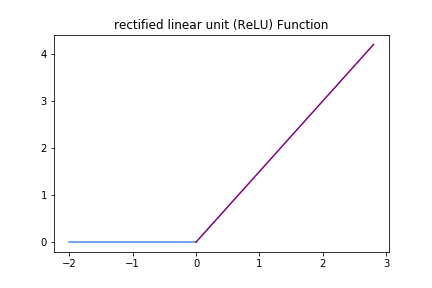
\includegraphics[width=0.4\textwidth]{fig/relu}
\end{figure}\begin{figure}[H]
	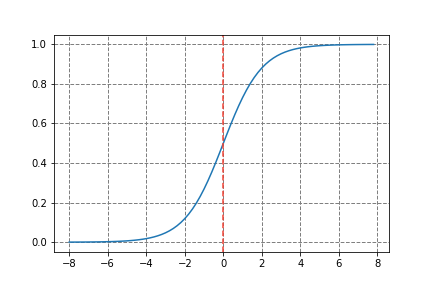
\includegraphics[width=0.4\textwidth]{fig/sigmoid}
\end{figure}}
\begin{python}
# Chapter 3 Pre-lecture Exercise
# 第三章课前练习
# @ Michael

# Import essential packages
# 导入必要扩展

import numpy as np
import matplotlib.pyplot as plt

# Play with colours in Python
# 简单的颜色绘图
# We will use matplotlib to plot a very simple function 
# with varied colours
# 我们将会使用 matplotlib 绘制简单的方程图形并且调试不同颜色

plt.plot([2], [3], 'bo')
plt.plot([4], [4], 'ro')
plt.plot([5], [2], 'go')
plt.axis([0, 6, 0, 7])  # change the range of axis
plt.grid(color='gray', linestyle='--', linewidth=1)  # add grid
plt.title('My first plot')


# plot ReLU function
x1 = np.arange(-2, 0.2, 0.2)
x2 = np.arange(0, 3, 0.2)
plt.plot(x1, 0*x1, color=(70/255, 136/255, 241/255))
# RGB(70, 136, 241)
plt.plot(x2, 1.5*x2, 'purple')
plt.title('rectified linear unit (ReLU) Function')


# plot sigmoid function
x3 = np.arange(-8, 8, 0.2)
y3 = np.exp(x3)/(1+np.exp(x3))
plt.plot(x3, y3)
plt.grid(color='gray', linestyle='--', linewidth=1)  # add grid
plt.axvline(x=0, color=(243/255, 66/255, 53/255), linestyle='--')
# add vertial line
\end{python}
\noindent
\textcolor{blue}{三色图结构}:
下面Python编程是对图片的数字化解构,这一部分程序的运行我们在\textbf{编程练习课中会进一步讲解},因此预习该部分时,稍微浏览即可,无需深入探究。另外,课堂中我们还会进一步探究图片的存储结构和颜色结构,所以请`稍安勿躁'。\mn{计算机图形学已经成为一门独立的学科,而且是一个很庞大的产业。比如苹果的创始人之一Steve Jobs(乔布斯)最初设立苹果公司的初衷就是想要一款可以显示精美字体的计算机,而不是他认为很`丑陋’的windows。如果经常浏览国外网站的同学可能会注意在网页审美设计上,我们还有很大的进步空间。比如浙大的官网,就让人觉得该校的网页设计专业可能不会太好,否则设计的网站不会如此的让人怀疑自己是否具有`信息密集恐怖症'。不过如此的传统也有好处,就是你会发现中国很多的网页设计都像是`头条’设计,一个方框内放一排排的文字再陪一张图片(喝一瓶娃哈哈,解解渴吧)。\textbf{特别提醒}:我们在Python环境下进行图片处理时,优选jpg格式,尽量避免使用png格式。具体的原因和不同情况下的转换,我们会进一步讲解。}
\begin{python}
# Chapter 3 Pre-lecture Exercise
# 第三章课前练习
# @ Michael

# Import essential packages
# 导入必要扩展

import numpy as np
import matplotlib.pyplot as plt
import matplotlib.image as mtmg

# Discover images (探索图片)
# We will import two images and explore how computer store and display images
# 我们将会读取两张图片来探索计算机是如何存储和显示图片的

# The cute panda 可爱的大熊猫
im_panda = mtmg.imread(
    '/Users/Michael/Documents/MDLforBeginners/Chapter3/Code/Images/panda.JPG')
# read panda image 熊猫图片读取
plt.imshow(im_panda)  # show image, 图片显示

im_panda.shape  # (1400, 1400, 3)
print(type(im_panda))   # <class 'numpy.ndarray'>
print(im_panda[:10, :10, 1])  # print 10 by 10 matrix in the second layer
plt.imshow(im_panda[:, :, 0], cmap='gray')
plt.imshow(im_panda[:, :, 1])
plt.imshow(im_panda[:, :, 2])
print(im_panda[700:710, 700:710, 0])
print(im_panda[700:710, 700:710, 1])
print(im_panda[700:710, 700:710, 2])

fig, ax = plt.subplots(nrows=1, ncols=3, figsize=(15, 9))
for i, ax in zip(range(3), ax):
    split_temp = np.zeros(im_panda.shape, dtype='uint8')
    split_temp[:, :, i] = im_panda[:, :, i]
    ax.imshow(split_temp)


# The Mosaic Painting 马赛克绘画
# prefer jpg format, rather than png format
im_mosaic1 = mtmg.imread(
    '/Users/Michael/Documents/MDLforBeginners/Chapter3/Code/Images/Mosaic1.jpg')
plt.imshow(im_mosaic1)
im_mosaic1.shape  # (1034, 1562, 4)
print(im_mosaic1[:10, :10, 1])
plt.imshow(im_mosaic1[:, :, 0])
print(im_mosaic1[700:710, 700:710, 0])
print(im_mosaic1[700:710, 700:710, 1])
print(im_mosaic1[700:710, 700:710, 2])

fig, ax = plt.subplots(1, 3, figsize=(15, 9))
for i, ax in zip(range(3), ax):
    split_temp = np.zeros(im_mosaic1.shape, dtype='uint8')
    split_temp[:, :, i] = im_mosaic1[:, :, i]
    ax.imshow(split_temp)


# The RGB Mosaic
# 三色马赛克
im_rgbmosaic = mtmg.imread(
    '/Users/Michael/Documents/MDLforBeginners/Chapter3/Code/Images/rgbmosaic.jpg')
plt.imshow(im_rgbmosaic)
im_rgbmosaic.shape

# pin down the red color
print(im_rgbmosaic[500:520, 600:620, 0])
print(im_rgbmosaic[500:520, 600:620, 1])
print(im_rgbmosaic[500:520, 600:620, 2])
plt.imshow(im_rgbmosaic[500:520, 600:620, :])

# pin down the blue color
print(im_rgbmosaic[500:520, 230:250, 0])
print(im_rgbmosaic[500:520, 230:250, 1])
print(im_rgbmosaic[500:520, 230:250, 2])
plt.imshow(im_rgbmosaic[500:520, 230:250, :])

# pin down the green color
print(im_rgbmosaic[800:820, 830:850, 0])
print(im_rgbmosaic[800:820, 830:850, 1])
print(im_rgbmosaic[800:820, 830:850, 2])
plt.imshow(im_rgbmosaic[800:820, 830:850, :])	
\end{python}
\noindent
\textcolor{purple}{反馈统计}:请扫描右边二维码,回答对此次课前预习的评估,只有三个问题。Michael 表示非常感谢,请同学多多配合。老师会根据你们的反馈对下一次C1进行提升和改进。填问卷的时候记得喝一杯茶或者咖啡$\heartsuit$。 \begin{marginfigure}
	\centering
	
\includegraphics[width=\textwidth]{fig/C3C1qrcode}
\end{marginfigure}


\newpage

\subsection{课堂讲义C2}

从这一小章节开始,我们开始进一步学习神经网络模型。按时完成C1的同学,或许已经对人工智能的广泛应用和蓬勃发展已经有了一定的了解。那么接下来,我们就开始系统学习或者说系统训练你们的`人工智能’思维。\textbf{因为这是高中课程,所以我的授课重点是训练你用人工智能解决问题的思维方式}, 在此基础上教授你相应的编程工具。本章节的学习重点有:
\begin{itemize}
	\item 何谓一般的`学习过程’
	\item 传统的问题解决方式和人工智能的解决方式有什么不同
	\item 大数据对人工智能的意涵是什么
	\item 标准神经网络学习模型的组成结构
\end{itemize}

\subsubsection{学习过程的一般性原理}

\begin{fullmodel}
	我们在C1的哲学延伸中(p.2)给出了一个简单的学习过程,即你第一次感受到烫伤后的行为调整过程。同学们可以回忆下自己第一次学自行车,或者第一次使用手机等学习过程中,都包括以下三个基本过程:
	\begin{itemize}
		\item 认知对象(问题)的接触,认知感觉和经验的揽集;
		\item 调用已有概念或知识对所在的场景进行分析;
		\item 做出判断和行动指令,并且有所行动。\begin{itemize}
		\item 如果所做判断和行动,符合预期目标,则维持;
		\item 否则进行修正和调整
		\end{itemize}
	\end{itemize}
	
对以上的学习和认知过程,我们简单概况为一个认知框架:
\begin{figure}[H]
	\centering
	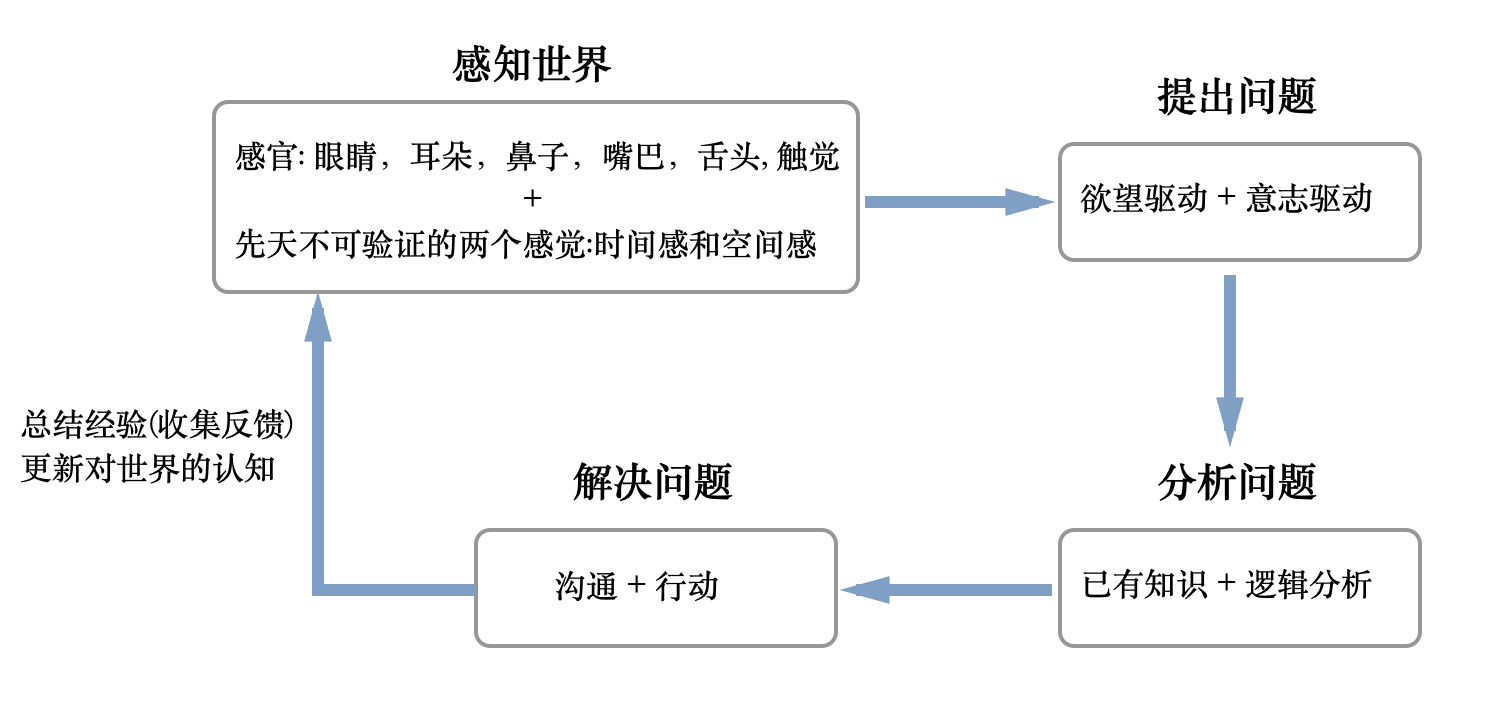
\includegraphics[width=0.69\textwidth]{fig/epismeflow}
\end{figure}

传统的问题解决方法和人工智能解决方法都符合以上框架,但是两者在对具体问题的解决上\textbf{有很大的不同}!
\end{fullmodel}

\subsubsection{传统问题解决方式 VS. 人工智能问题解决方式}

传统的问题解决方式和人工智能问题解决方式最大的不同体现在以下两个方面:
	\begin{itemize}
		\item 传统的问题解决方式着重对问题进行分步骤拆解和处理;
		\item 人工智能对问题的解决方式着重对整个流程的两个端口进行数据和模型联通。
	\end{itemize}
我们通过具体的三个个案例来进行详细的分析,案例一是有关商业广告的投放,案例二是有关信用卡违约,案例三是谷歌AlphaGo(阿尔法狗)的`blackbox'(黑箱)模式。

\definecolor{deepramp}{RGB}{104, 25, 65}

\noindent
\textcolor{deepramp}{案例一} 商业广告投放: 传统的商业广告投放在确定了目标客户后,会通过各种方式(比如问卷调查,消费行为习惯,心里图谱鉴定)对客户群体通过一些列数据来描述。根据所收集的数据建立相应的模型。这些模型的建立往往经由专业人士,比如管理学毕业的学生,或者经济学毕业的学生来完成。决策者在收集数据和模型建立后,然后进行广告的投放。然而,人工智能下的问题解决框架仍然需要收集大量数据,不过由于数字经济方兴未艾,所以数据的收集变得更加容易。收集数据后,对于广告投放的模型构建上,就不需要太多得研究,因为我们可以选择深度学习模型(deepmind model)让计算机自己去学习。\textbf{机器具体如何学习,是我们本章节的重点内容}。

\hfil

\noindent
\textcolor{deepramp}{案例二} 信用卡违约:传统信用卡违约的解决,同样需要进行数据收集,然后银行会聘用专业的风险分析师或者精算师,来进行模型的构建。这些模型的构建往往需要概率论和统计学的系统训练。比如精算师会根据不同场景进行风险的计算,然后指导银行进行信用卡的管理。人工智能是在收集大量数据的基础上,对于相关模型进行训练,然后指导银行进行信用卡管理。我们会在课上,进一步讲解机器是如何学习的。

\hfil

\noindent
\textcolor{deepramp}{案例三} AlphaGo: 2016年阿尔法狗战胜之后,科学美国人杂志(Scientific American)采访AlphaGo的设计人员,邀请他们介绍DeepMind(深度神经网络)为什么能够打败人类顶尖棋手。设计人员可以接受他们模型的构造原理,但是具体这个模型内部的运行过程,他们经常戏称为`黑箱作业'(Black Box)。我们会在本节课中解释他们所称的黑箱是何物。科学美国人原文链接:\url{https://www.scientificamerican.com/article/demystifying-the-black-box-that-is-ai/}


\subsubsection{神经网络模型机制}

\begin{fullmodel}
	教材中有两张图片,即图3-15和图3-19,给出了神经网络模型的工作流程。我们把两个图片中的模型进行简化,绘制下面这张流程图(来源:斯坦福大学深度学习官网)。
\begin{figure}[H]
	\centering
	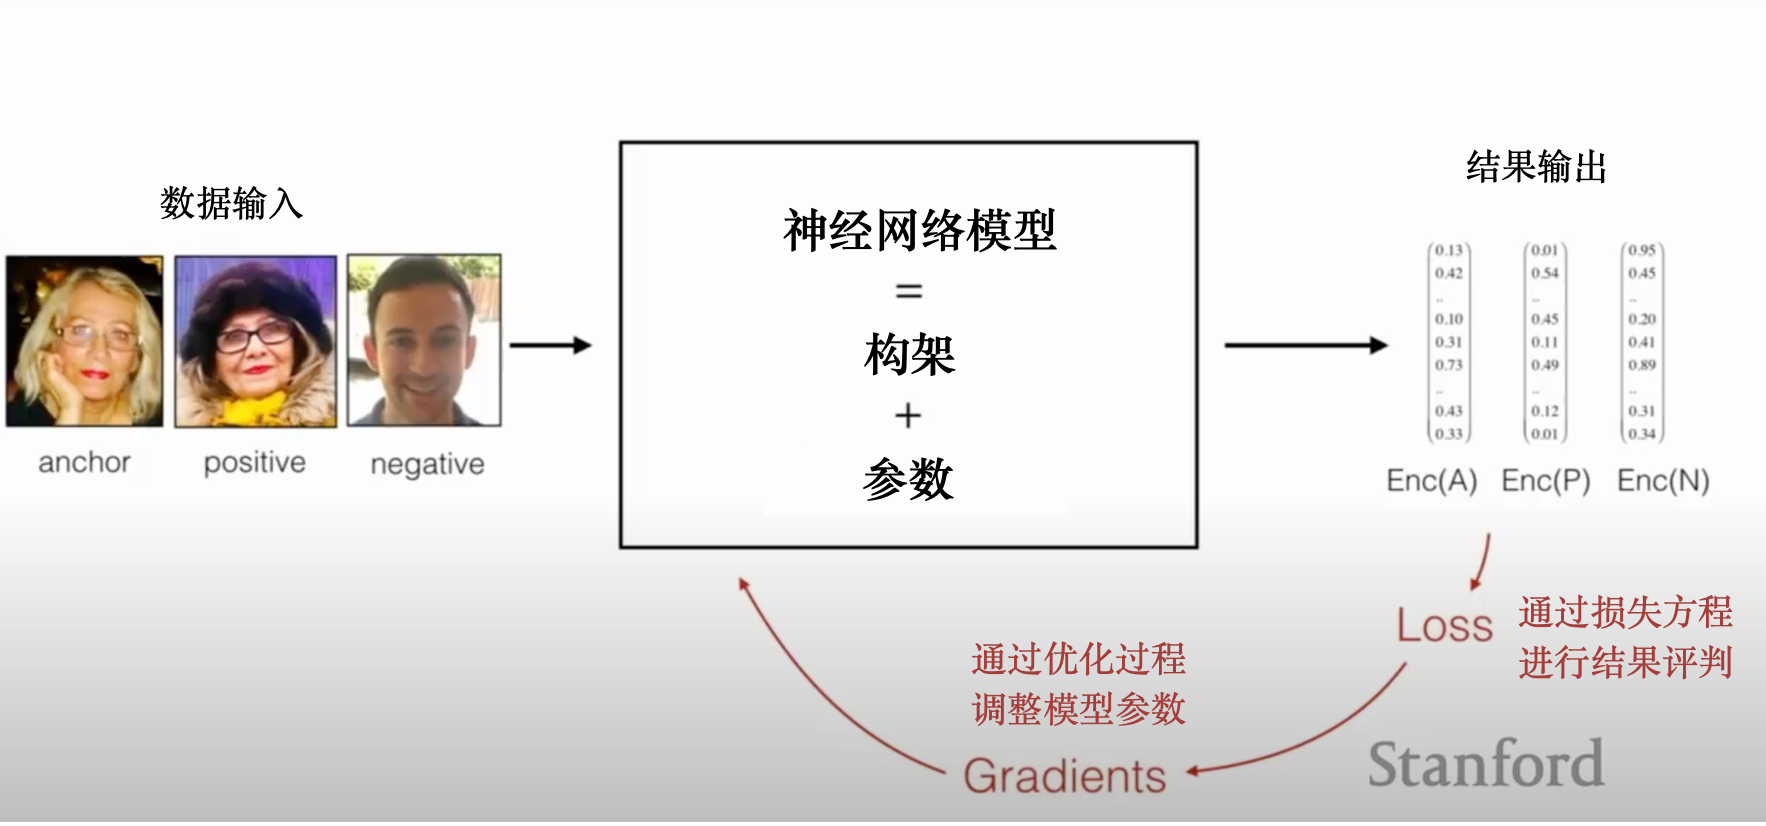
\includegraphics[width=0.8\textwidth]{fig/deepmindflow}
	\caption{深度学习简要框架}
\end{figure}
深度模型的构建的基本单元是一连串的函数组合,这些函数的线性组合构成了我们所称的`神经网络'以及卷积(convolution)的过程。了解这些函数的作用以及卷积的过程对于理解深度学习网络至关重要。所以我们会花费比较多的时间来讲解这些数学概念。
\end{fullmodel}

\subsubsection{数据结构}

因为机器学习和人工智能需要大量的数据,所以非常有必要对数据结构进行定义和分类\mn{生活中最常见的数据形式应该是Excel表格。}。

\begin{definition}
	我们把由数字和对其的描述(有其根据)组成的信息形态,称为\textit{数据};我们将统一在一个描述下的数列,称为\text{数据集}; 有多个数据集构成的一系列数据,称为\textit{数据阵}。
\end{definition}
\begin{marginfigure}
	\centering
	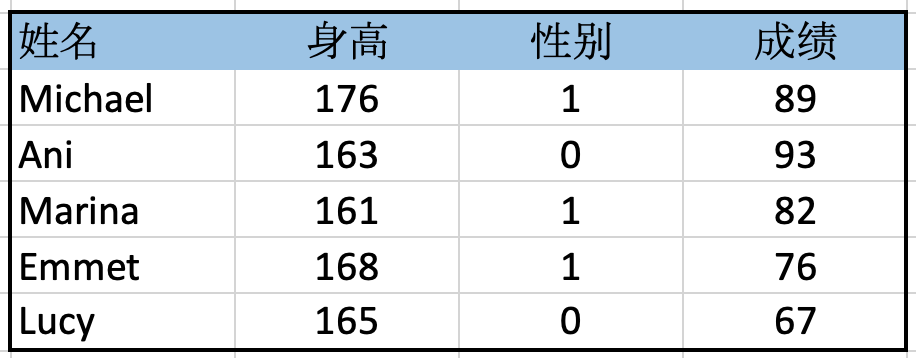
\includegraphics[width=0.9\textwidth]{fig/dataframeEx}
\end{marginfigure}
\begin{remark}
很显然,如果我只给你一个数,比如6, 我们不能称其为数据,因为其缺乏对其的描述。比如,`年方二八’, 年龄16岁,则可以成为数据。	再比如,2019 不是数据,2019年则是数据。
\end{remark}

\begin{example}
数据: 红色-255; 数据集: 颜色: 红255, 绿666, 蓝521; 数据阵:[[颜色:190, 321, 589]; [年份:2019, 2020, 2056]]。右边的表格就是一个数据阵。数据阵(dataframe)是Python和R语言中常用的数据形式。
\end{example}

\begin{definition}
	我们把语言文本,网页信息,图片和影音等的复合数据,称为\textit{多媒体数据集}。
\end{definition}

\begin{example}
下面这张图片是由 Peggy Collins 创作的马赛克数字图画。这张图片在计算机中的存储形式是具有维度$(1400, 1400, 3)$的数据集构成。其中3,是代表的RGB(红绿蓝)三层底色层,每一个色素层是由一个$1400 \times 1400$的矩阵组成。
\begin{figure}[H]
	\centering
	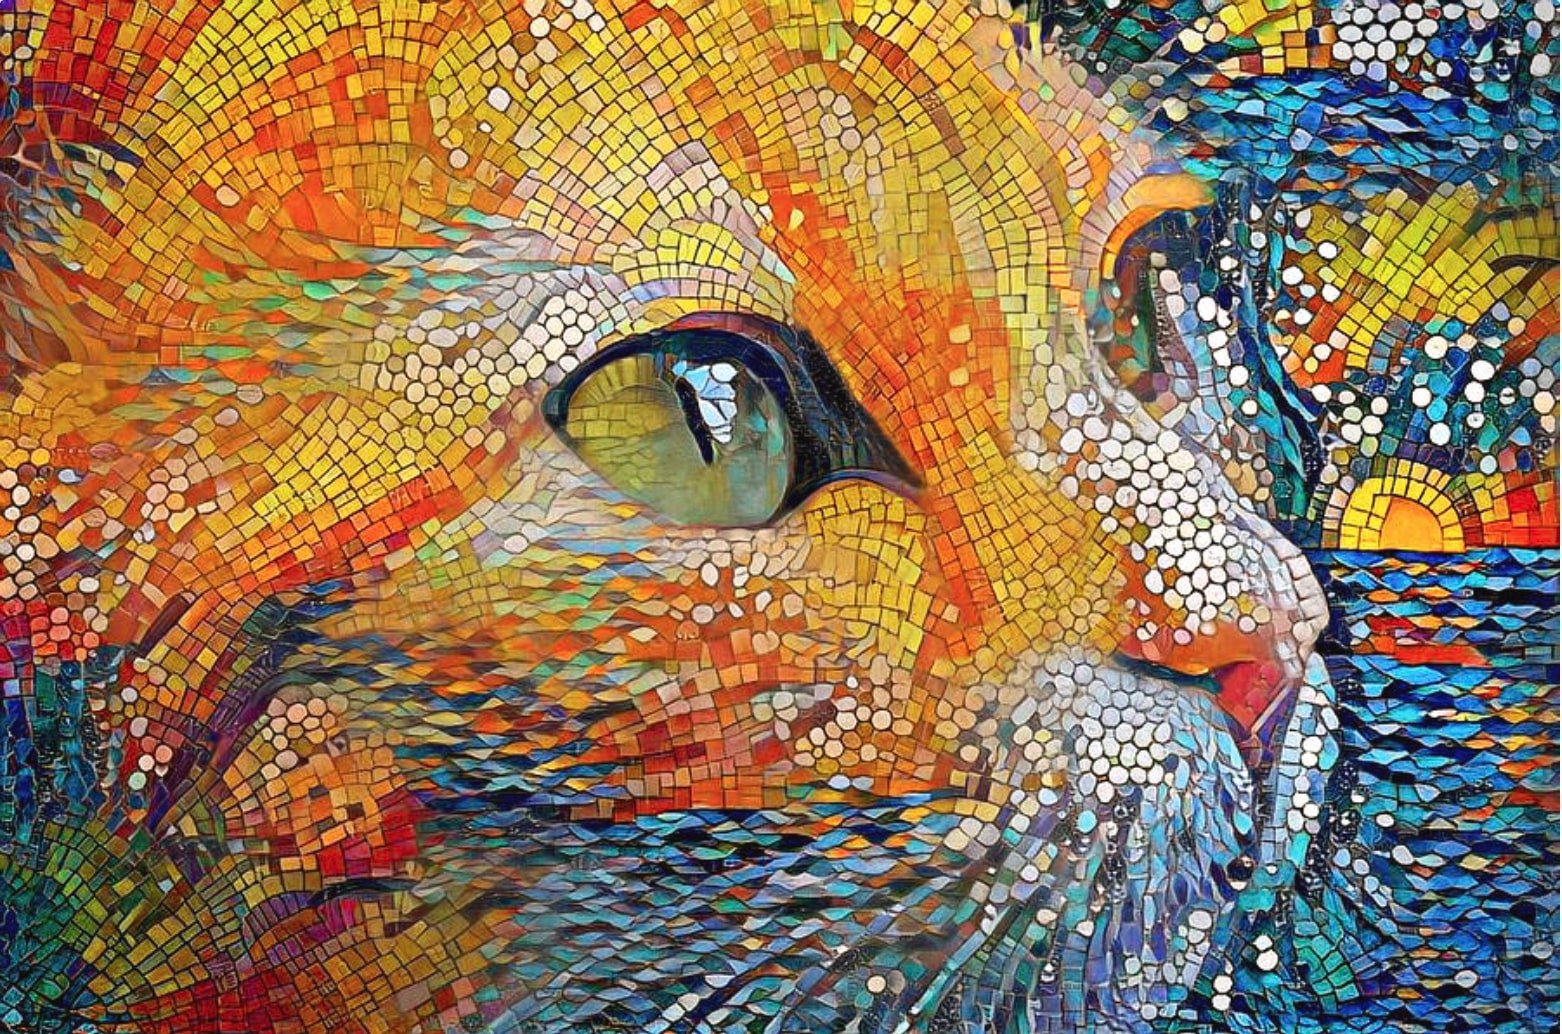
\includegraphics[width=\textwidth]{/Users/Michael/Documents/MDLforBeginners/Chapter3/Code/Images/Mosaic1.jpg}
	\caption{Ginger Cat by Peggy Collins (digital artwork)}
\end{figure}	
\begin{python}
print(im_mosaic1[:10, :10, 1])
# [[246 190 116  51  30  21   0   6  28  42]
#  [188  88  48  52  40  20   4  12  28  39]
#  [108  40  37  55  43  27  17  15  24  35]
#  [ 35  34  41  39  35  32  21  18  21  31]
#  [ 20  24  25  26  34  26  13  23  23  29]
#  [ 35  25  24  29  28  19  17  26  25  29]
#  [ 28  23  24  22  15  17  24  22  23  25]
#  [ 33  29  18  15  18  17  15  12  18  19]
#  [ 18  14  13  16  19  19  19  18  15  11]
#  [  8   6   8  16  23  26  24  21  20  15]]	
\end{python}
\end{example}

\begin{definition}
	我们将多媒体数据集和数据阵组合构成的数据形态成为\textit{数据群}或者\textit{大数据}。数据群或大数据,在业界也被称为\textbf{有标注的数据群}。
\end{definition}

\begin{example}
比如,下面这个数据群,就是一个有标注的数据群。\mn{大数据时代,数据的标注准确度和密集度,成为衡量数据群质量的重要指标。国际上,目前美国的数据群质量最高,其次是英国和德国。中国的数据群目前取胜于量,对于质的追求,还需要一定的时间。}
\begin{table}[H]
	\centering
	\renewcommand{\arraystretch}{1.5}
	\begin{tabular}{ccccc}
	\hline 
		图片(1400, 1400, 3) & 年份 & 地点 & 备注1 & 备注2 \\
		\hline 
		图1 & 2016 & 桥 & 青岛 & 红色 \\
		图2 & 2020 &  伦敦 & 人 & 女 \\
		图3 & 2013 & 成都& 熊猫 & 国宝\\
		\hline 
	\end{tabular}
\end{table}
\end{example}


\subsubsection{损失方程(Loss Function)}

人工智能中很多模型,包括神经网络学习模型都需要有标注的数据群。比如我们通过想要训练神经网络学习模型辨别图片中的人物的性别,那么就需要具有\textit{性别标注}的图片数据群。拥有了标注的数据,就可以训练人工智能模型,从而可以调整模型参数,来提升预测准确度。而用来衡量准确度的方程就需要损失方程。

\begin{definition}
	假设数据群标注过的数据准确可靠,在人工智能模型中,模型在整合输入数据且加工计算后输出的结果与数据群标注的数据差别的方程称为\textit{损失方程(Loss Function)}。
\end{definition}

\begin{example}
比如我们想要通过人工智能来判定图片中人类的性别,下面的表格中给出了最为简单的一种损失方程。
\begin{table}[H]
	\centering
	\renewcommand{\arraystretch}{1.5}
	\begin{tabular}{cccc}
	\hline 
		图片(1400, 1400, 3) & 标注(1-男,0-女) & 模型预测 & 差异\\
		\hline 
		图1 & 1 & 0 & 1 \\
		图2 & 0 & 1 & 1 \\
		图3 & 1 & 1 & 0 \\
		\hline 
	\end{tabular}
\end{table}
用$\hat{Y}$来代表预测的结果,$Y$来代表标注结果,那么损失方程为:
\begin{align*}
	L(Y, \hat{Y}): |Y-\hat{Y}| 
\end{align*}
\end{example}

\begin{remark}
损失方程(Loss function) 有很多设计。设计或者选择损失方程的依据是为了更好得训练人工智能的模型,从而提升预测准确度。后面我们还会逐渐介绍不同的损失方程,但是其一般形式为:
\begin{align*}
	L: (Y, \hat{Y}): \ \to \rn 
\end{align*}	
\end{remark}

\subsubsection{初始数据群处理}

在具体的人工智能实践中,我们很多时间实际上是花在处理初始数据群上的\mn{Data scientists spend 80\% of their time cleaning data rather than creating insights.}。这是因为初始数据群的整洁程度和能否直接被人工智能模型接受,会影响我们后面对模型的训练和各类模型的调试。因为处理初始数据群非常重要,所以很多公司会聘请专门的数据专家进行数据整理和矫正。希望同学们在具体的操作中,也有数据集群意识。因为本章的神经网络模型处理较多的是图片,所以我们接下来重点介绍图片的多媒体数据集合构成。


\subsubsection{向量、矩阵和其相关的运算}

无论是\textit{多媒体数据集}还是\textit{数据阵},除去其标注的信息,具体的数都是储存在矩阵中的。

\begin{definition}
	\textit{矩阵}(Matrix)是一个按照长方阵列排列的复数或实数集合。对一个矩阵的简单描述可以为 $m \times n$ 的矩阵,即该矩阵有$m$ 行,$n$列. $m \times n$也被称为矩阵的大小。
\end{definition}
\begin{example}
比如,我们有$3 \times 3 $的矩阵$A$ 和$2 \times 3$ 的矩阵$B$。
\begin{align*}
	 A = \begin{bmatrix}
	1 & 3 & 4 \\
	2 & 5 & 8 \\
	3 & 9 & 7
\end{bmatrix}, & & B = \begin{bmatrix}
	3.2 & 1.9 & 5.7 \\
	4.1 & 5.8 & 9.3 \\
\end{bmatrix}
\end{align*}	
\end{example}

\begin{definition}
	矩阵中单独的一行被成为\textit{行向量}(row vector), 单独的一列别成为\textit{列向量}(column vector)。
\end{definition}
\begin{example}
比如在上面的矩阵$A$中,	我们有以下单独的向量:
\begin{align*}
	A_{r2} = [2 \ 5 \ 8],  & & A_{c2} = \begin{bmatrix}
		3 \\
		5 \\
		9 
	\end{bmatrix}
\end{align*}
\end{example}

\begin{definition}
	现有同样大小的$m \times n$的矩阵 $A, B$, 我们定义矩阵的加法($+$)运算为:
	\begin{align*}
		A + B = \begin{bmatrix}
			(a_{11} + b_{11}) & (a_{12}+b_{12}) & \cdots & (a_{1n}+b_{1n}) \\
			a_{21} + b_{21} & a_{22}+b_{22} & \cdots & a_{2n}+b_{2n} \\
			\vdots & \ddots & & \vdots \\
			a_{m1} + b_{m1} & a_{m2}+b_{m2} & \cdots & a_{mn}+b_{mn} \\
		\end{bmatrix}
	\end{align*}
	其中,$a_{ij}$ 为矩阵$A$中第$i$行第$j$列元素,$b_{ij}$ 为矩阵$B$中第$i$行第$j$列元素。
\end{definition}

\begin{remark}
矩阵的加法只能在同样大小的矩阵中进行,即同位元素相加。	
\end{remark}

矩阵最早的提出是为了解决多项式的求解,比如下面方程组的转换。
\begin{align*}
	2x_1 + 3x_2 + 7x_3 & = 9 \\
	4x_1 + 5x_2 + 8 x_3 & = 10 \\
\end{align*}
可以用矩阵的乘法来表示:
\begin{align*}
	\begin{bmatrix}
		2 & 3 & 7 \\
		4 & 5 & 8 
	\end{bmatrix} \begin{bmatrix}
		x_1 \\
		x_2 \\
		x_3 
	\end{bmatrix} = \begin{bmatrix}
		 9 \\
		 10 
	\end{bmatrix}
\end{align*}

\begin{definition}
	现有$m \times n$ 的矩阵A 和 $n \times k$的矩阵$B$, 我们定义矩阵的乘法$\cdot$为
	\begin{align*}
		(A \cdot B)_{ij} = \sum_{r=1}^n a_{ir}b_{rj} = a_{i1}b_{1j} + a_{i2}b_{2j} + \cdots + a_{in}b_{nj}
	\end{align*}
	其中$(A \dot B)_{ij}$是两个矩阵相乘后的第i行第j列元素。
\end{definition}

\begin{remark}
取任意$a \times b$ 矩阵A 和$c \times d$ 矩阵 B, 如果$b \neq c$,则两个矩阵不可以相乘。	
\end{remark}

\begin{example}
计算下列矩阵的乘法
\begin{align*}
	\begin{bmatrix}
		2 & 3 & 7 \\
		4 & 5 & 8 
	\end{bmatrix} \begin{bmatrix}
		1 \\
		0 \\
		-1 
	\end{bmatrix} = \ ? & & \begin{bmatrix}
		1 & 3 & 3 \\
		2 & 8 & 4 \\
		3 & 9 & 1 
	\end{bmatrix} \begin{bmatrix}
		3 & 2 \\
		1 & 0 \\
		-1 & 8 
	\end{bmatrix} = \ ?
\end{align*}	
\end{example}

\subsubsection{卷积运算(Convolution)}

卷积运算(Convolution)是图形处理中特有的一种运算方式。其目的是\textbf{系统性一次性得}对原始图片进行快速处理。我们之前已经讲解过图形的储存形式,而且在课前预习中的习题中也特别对卷积运算进行了铺垫,接下来我们就更加规范得对这个概念进行学习。

\begin{definition}
	给定一个长度为$m$的向量$A$和一个长度为$n$的向量$B$, 其中$n > m$:
	\begin{align*}
		A & = [a_1, a_2, \cdots, a_m ] \\
		B & = [b_1, b_2, \cdots, \cdots, a_n]
	\end{align*}
	我们称$A$为\textit{参数(核)向量}\mn{kernel vector},$B$为\textit{数据向量},其卷积运算(convolution)$*$定义为
	
	\begin{algorithm}[H]
	\SetAlgoLined
	\caption{Convolution Operation}
	初始化长度为$n-m+1$的向量$C = [c_1, c_2, \cdots, c_{n-m+1}]$ \;
	$C = A * B $ \; 其中,每一个元素的计算方法为\;
	\For {$i \ in \ [1:n-m+1]$}{$c_i = \sum_{k=1}^m a_k b_{k+i-1} = a_1 b_i +  a_2 b_{i+1} +\cdots + a_m b_{i+m-1}$}
	\end{algorithm}
\end{definition}

\begin{example}
	现有参数向量$A=[1, 3, 4]$ 和数据向量$B = [5, 6, 7 , 8 , 9]$,那么
	\begin{align*}
		A * B & = [34, 40, 46]\\
		34 & = 1\times 5 + 3 \times 6 + 4 \times 7 \\
		40 & = 1 \times 6 + 3 \times 7 + 4 \times 8 
	\end{align*}
\end{example}

\begin{definition}
	给定一个$m \times n$的矩阵$A$,和一个$k \times l$的矩阵$B$,并且$k > m, l > n$, 那么矩阵$A$被叫作\textit{参数(核)矩阵}\mn{kernel matrix},矩阵$B$被称为\textit{数据矩阵}。那么矩阵$A$和$B$的卷积运算定义为
	\begin{align*}
		A * B = \text{移动参数向量对数据向量进行对位求积后求和}
	\end{align*}
	运算过程如下图所示(来源:Irhum Shafkat, 2018)\mn{矩阵的卷积有很多种,更多的介绍请参考该网站:\url{https://towardsdatascience.com/intuitively-understanding-convolutions-for-deep-learning-1f6f42faee1}}。
\end{definition}

\begin{figure}[H]
	\centering
	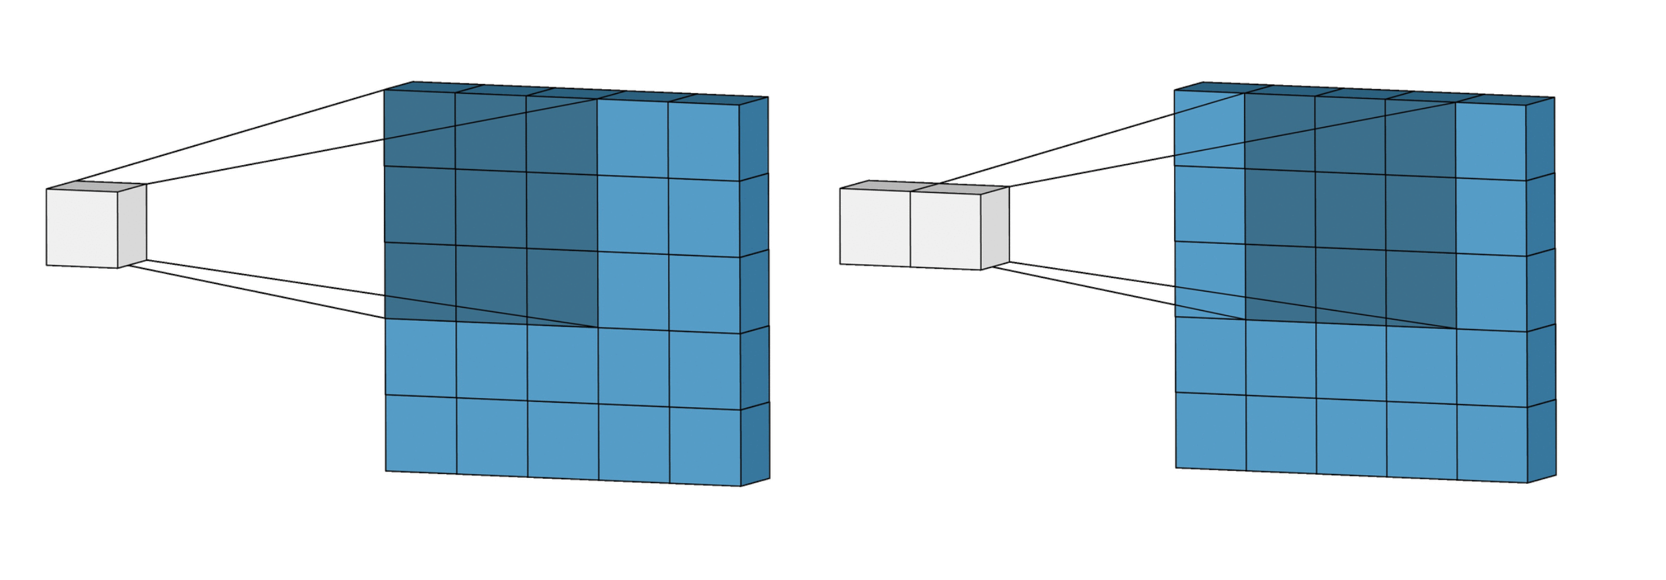
\includegraphics[width=\textwidth]{fig/mtconvo}
	\caption{基本矩阵卷积计算}
\end{figure}

\begin{remark}
	矩阵的卷积运算目的是想要通过参数矩阵来对数据矩阵进行进一步的处理。之所以需要这个处理过程是因为
	\begin{itemize}
		\item 原始多媒体数据集维数较大,比如图3.4中的猫有$(1400, 1400, 3)$,即$1400 \times 1400 \times 3 = 588000$个数(元素)组成。通过卷积运算后数据集的维数会有所下降,从而节省模型训练时间;
		\item 原始多媒体数据集的特征不明显,需要通过参数矩阵的卷积运算后来进行优化;
		\item 卷积在图像识别中的应用原因还有其它的,以后我们会结合具体案例进一步讲解。\mn{卷积运算主要应用在图像识别中,在其它领域,比如金融数据的人工智能模型,则没有被那么广泛得使用。}
	\end{itemize}
\end{remark}

\begin{example}
我们手动计算一种标准的卷积形式,给定参数核矩阵$A$和数据矩阵$B$为
\begin{align*}
	A = \begin{bmatrix}
		1 & -1 \\
		1 & 2 
	\end{bmatrix} & & B= \begin{bmatrix}
		1 & 2 & 1 \\
		2 & 3 & 6 \\
		0 & 5 & 7 
	\end{bmatrix}
\end{align*}	
我们演示计算结果矩阵($C = A*B$)的第一个元素\mn{$C=A*B$的最终结果为\begin{align*}
	C = \begin{bmatrix}
		7 & 16 \\
		9 & 16
	\end{bmatrix}
\end{align*} 你会发现$C$中元素最大值是$16$,刚好在$B$的右下角,这是巧合吗?(显示不是,否则我也不发发问了)}
\begin{align*}
	C_{11} = 1\times 1 + (-1) \times 2 + 1 \times 2 + 2 \times 3 = 7 
\end{align*}
\end{example}


\begin{example}
为帮助同学们理解参数卷积的重要性,我们特别详细分析一个生活常见的具体案例。下面的表格是一个班级内几名同学的不同学科的成绩表,我们来计算不同的参数卷积矩阵可以给出不同的`评估'结果(这个评估结果可以理解成我们机器学习的一个运算结果)。
\begin{figure}[H]
	\centering
	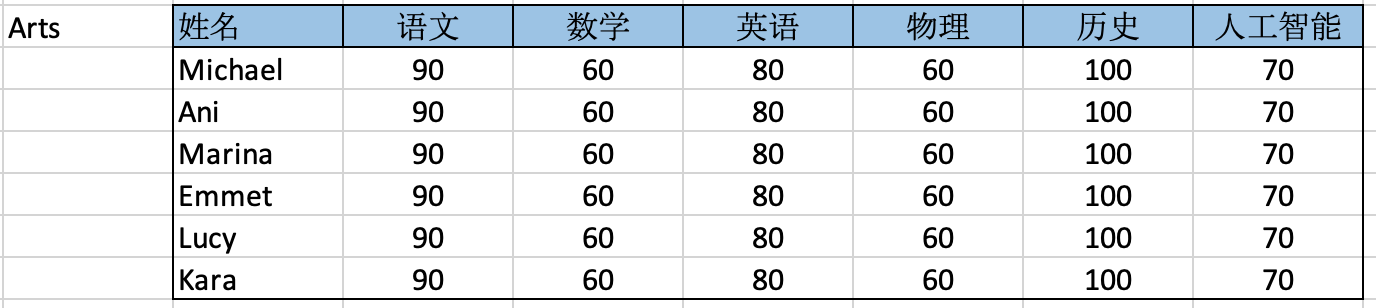
\includegraphics[width=\textwidth]{fig/artsgrade}
	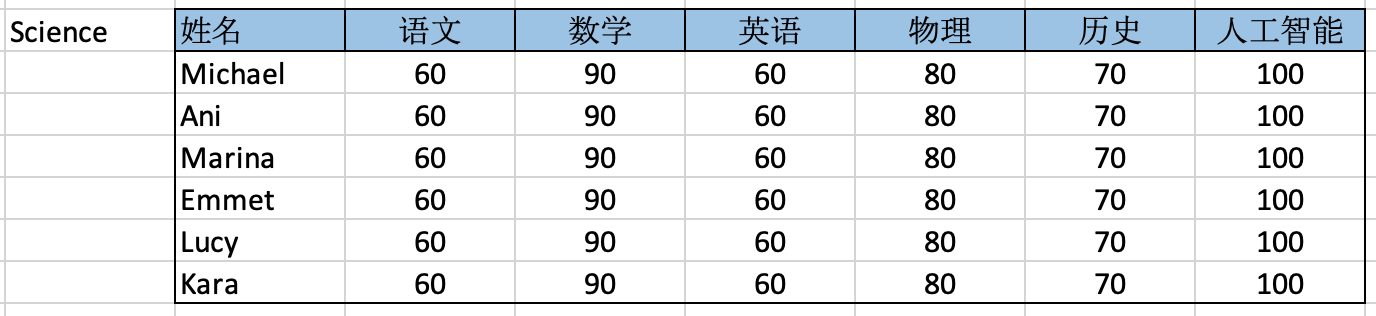
\includegraphics[width=\textwidth]{fig/sciencegrade}
\end{figure}
其中参数核(kernel)矩阵给定为
\begin{align*}
	K = \begin{bmatrix}
		1 & 0 & $-$1$$ \\
		1 & 0 & $-$1$$  \\
		1 & 0 & $-$1$$  
	\end{bmatrix}
\end{align*}
将文科生(arts)和理科生(science)的数据阵进行两次卷积运算:
\begin{align*}
	A \Rightarrow \begin{bmatrix}
		30 &    0  &   -60  &    -30 \\
       30  &     0  &    -60  &    -30   \\        
       30  &     0  &    -60  &   -30 \\
       30  &    0  &    -60  &   -30 
	\end{bmatrix} \Rightarrow \begin{bmatrix}
		270 & 90 \\
		270 & 90 
	\end{bmatrix} & & 	S \Rightarrow \begin{bmatrix}
	   0 & 30 & -30 & -60 \\
       0 & 30 &  -30 & -60 \\
        0 & 30 &  -30 & -60 \\
       0 & 30 &  -30 &  -60
	\end{bmatrix} \Rightarrow \begin{bmatrix}
		90 & 270 \\
		90 & 270 
	\end{bmatrix}
\end{align*}
两个矩阵看起来很相似,只是列向量顺序不同。如果我们将两个矩阵按照此前的顺序进行标注,可以得出下面的表格:\mn{如果你没有觉得数学像变魔术一样把复杂问题简单化的话,我也只能表示要喝一瓶王老吉了。}
\begin{table}[H]
\renewcommand{\arraystretch}{1.2}
	\centering
	\begin{tabular}{|l|cc|}
	\hline 
		学科/成绩集成 & 文科 & 理科 \\
		\hline 
		文科生& 270 & 90 \\
		& 270 & 90 \\
		\hline 
		理科生& 90 & 270 \\
		& 90 & 270 \\
		\hline 
	\end{tabular}
\end{table}
\end{example}

复杂神经学习模型要比以上的例子复杂的多,但是基本流程却非常相似,具体的计算和演化逻辑也可以说`如出一辙'。我们可以把神经网络深度学习的模型再一次概况为:\textbf{通过对输入端的数据群(大数据)进行标注和整理后,建立一个人工智能构架,并设定目标函数(损失方程),对所建立的构建(或模型)进行反复训练,直到找到符合我们目标函数要求的参数核矩阵。}

\noindent
下面是本讲内容使用的Python程序,有兴趣的同学可以自己复制后运行和进行改进调试。
\begin{python}
# Chapter 3 Lecture 1
# 课堂讲义
# @ Michael

# Import essential packages
# 导入必要扩展

import numpy as np
from scipy import signal

# vector convolution 向量卷积
a = np.array([1, 2, 3])
b = np.array([5, 6, 7, 8, 9])
np.convolve(a, b, 'valid')  # array([34, 40, 46])

# matrix convolution example 1
kernela = np.array([[1, -1], [1, 2]])
datamatrix = np.array([[1, 2, 1], [2, 3, 6], [0, 5, 7]])
print(signal.convolve2d(kernela, datamatrix, 'valid'))
# 注意该方程中的卷积方式,与我们定义的有所不同


def matrixConv(kenl, dtm):
    # Assume size of kenel is less than datamatrix
    # 假设参数核矩阵小于数据矩阵
    m = np.shape(kenl)[0]
    n = np.shape(kenl)[1]
    k = np.shape(dtm)[0]
    l = np.shape(dtm)[1]
    resltmtx = np.zeros([k-m+1, l-n+1])
    for i in range(resltmtx.shape[0]):
        for j in range(resltmtx.shape[1]):
            temp = 0
            for u in range(m):
                for p in range(n):
                    temp += kenl[u, p] * dtm[u+i, p+j]
                    resltmtx[i, j] = temp
    return(resltmtx)


# test the function
matrixConv(kernela, datamatrix)


# matrix convolution example 2
grade_arts = np.ones([6, 6])
grade_science = np.ones([6, 6])
grade_dist1 = [90, 60, 80, 60, 100, 70]
grade_dist2 = [60, 90, 60, 80, 70, 100]
for i in range(len(grade_dist1)):
    grade_arts[:, i] = grade_arts[:, i] * grade_dist1[i]
for j in range(len(grade_dist2)):
    grade_science[:, j] = grade_science[:, j] * grade_dist2[j]

print(grade_arts)
print(grade_science)

kernel_para = np.array([[1, 0, -1], [1, 0, -1], [1, 0, -1]])
conv_arts = signal.convolve2d(grade_arts, kernel_para, 'valid')
# array([[-30.,   0.,  60.,  30.],
#        [-30.,   0.,  60.,  30.],
#        [-30.,   0.,  60.,  30.],
#        [-30.,   0.,  60.,  30.]])
signal.convolve2d(conv_arts, kernel_para, 'valid')
# array([[270.,  90.],
#        [270.,  90.]])

# use self-wrote function
conv_arts2 = matrixConv(kernel_para, grade_arts)
# array([[ 30.,   0., -60., -30.],
#        [ 30.,   0., -60., -30.],
#        [ 30.,   0., -60., -30.],
#        [ 30.,   0., -60., -30.]])
matrixConv(kernel_para, conv_arts2)
# array([[270.,  90.],
#        [270.,  90.]])


conv_science = signal.convolve2d(grade_science, kernel_para, 'valid')
conv_science.shape
# array([[  0., -30.,  30.,  60.],
#        [  0., -30.,  30.,  60.],
#        [  0., -30.,  30.,  60.],
#        [  0., -30.,  30.,  60.]])
signal.convolve2d(conv_science, kernel_para, 'valid')
# array([[ 90., 270.],
#        [ 90., 270.]])

#use self-wrote function
conv_science2 = matrixConv(kernel_para, grade_science)
# array([[  0.,  30., -30., -60.],
#        [  0.,  30., -30., -60.],
#        [  0.,  30., -30., -60.],
#        [  0.,  30., -30., -60.]])
matrixConv(kernel_para, conv_science2)
# array([[ 90., 270.],
#        [ 90., 270.]])
\end{python}


Bonjour,我们这一节的课堂讲义就到此结束了,下面你要进行课后练习了。这些课后练习并不复杂,只是需要你动脑+动手。

\hfil

\noindent
\textcolor{purple}{疑难解答}:如果有相关疑问,请扫描下面的二维码,讲你的问题输入,老师会尽快答疑解惑:$\heartsuit$。 \begin{marginfigure}
	\centering
	
\includegraphics[width=\textwidth]{fig/C3C2qrcode}
\end{marginfigure}


\newpage
\subsection{课后练习C3}

\begin{fullmodel}
\begin{question}{思考题C3-Q1}
	Michael是一名研修植物学的大学生,他一直梦想只用通过手机拍照后,计算机就可以自动配图和文字,对他所拍的植物进行一份文档生成,而不是他亲自去采集植物,阅读资料,并且撰写有关植物学的报告。解决该类问题除了图像处理之外,还需要自然语言的处理。你认为他的梦想会在未来会实现吗?实际上,Michael爱好诗歌,他喜欢写短行诗后配上图片发到朋友圈上,下面是他发的一条朋友圈。请问你可以训练计算机写诗吗?
	\begin{figure}[H]
		\centering
		\begin{subfigure}[b]{0.45\textwidth}
			\centering
			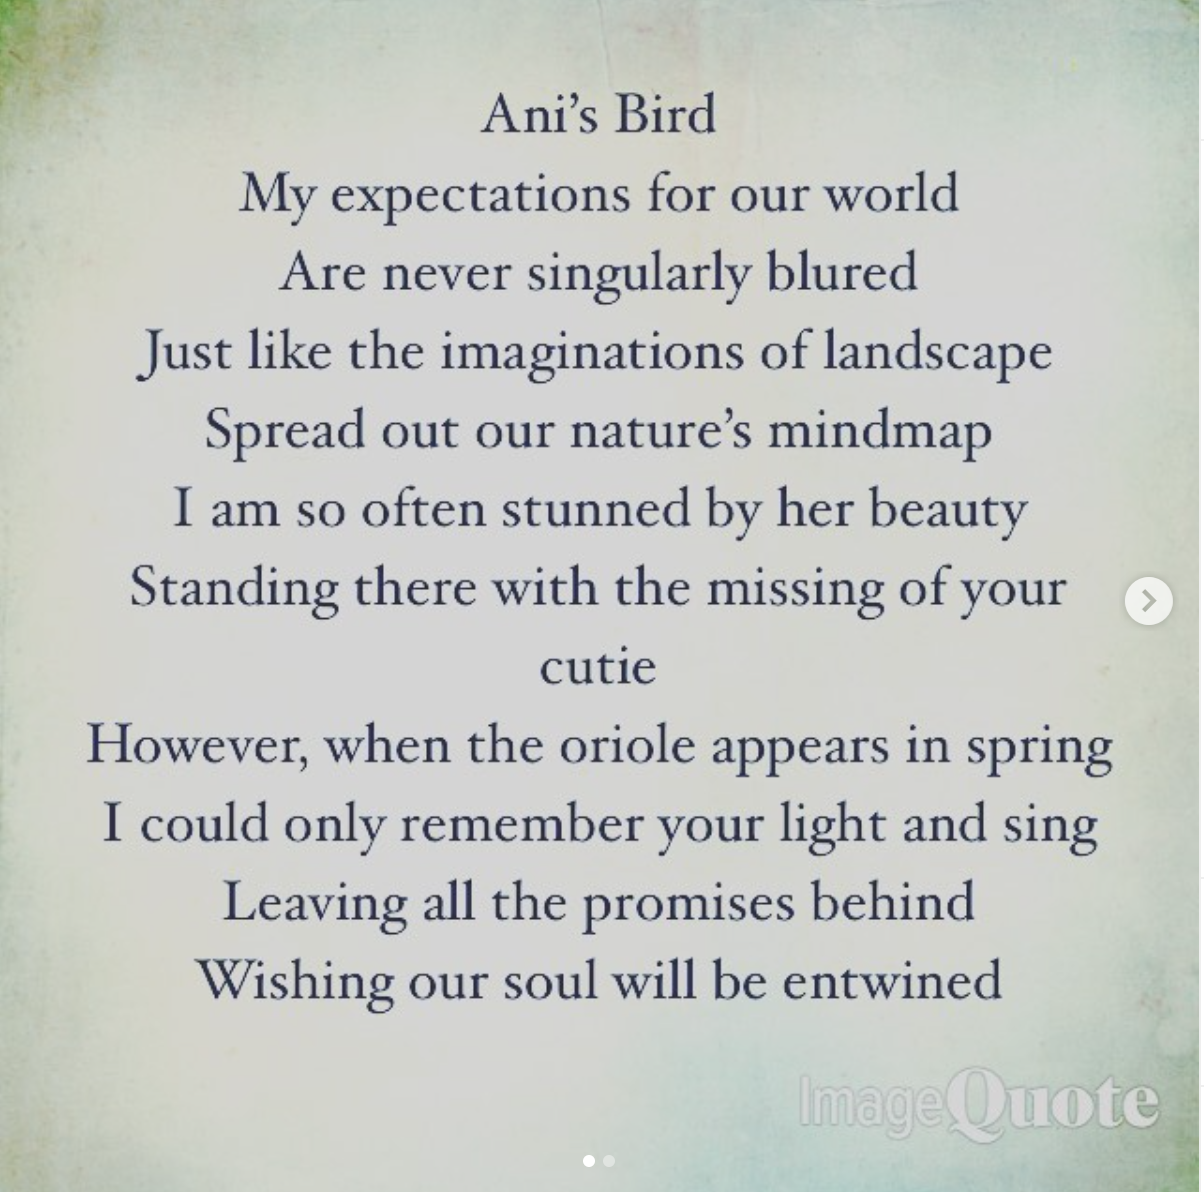
\includegraphics[width=\textwidth]{fig/poetry1}
		\end{subfigure}
		\begin{subfigure}[b]{0.45\textwidth}
			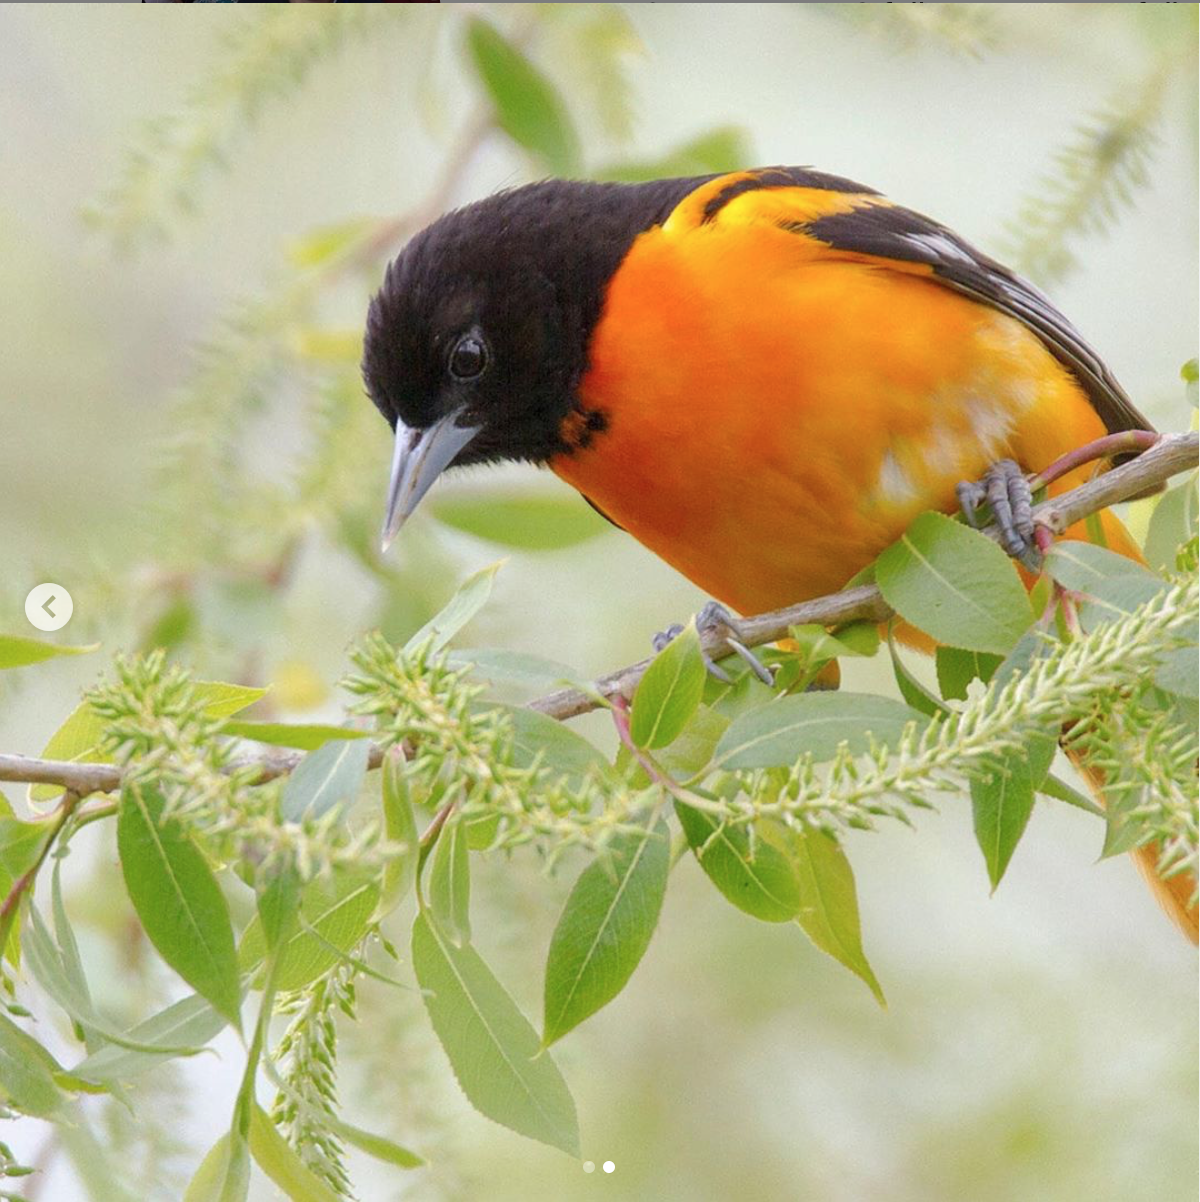
\includegraphics[width=0.99\textwidth]{fig/peotry2}
		\end{subfigure}
	\end{figure}
\end{question}	
\end{fullmodel}


\begin{fullmodel}
\begin{question}{设计题 C3-Q2}
	下面的表格中有九个描述,根据这九个描述,将你的数据构成一个$9 \times 9$的矩阵。然而设计一个损失方程(Loss function),然后计算你跟班里的同学谁最\textit{相像}。其中性别代码1指男性,0指女性。所有的数据均采用公有制单位,比如身高176cm,在矩阵中填176即可,视力1.5等
	\begin{figure}[H]
		\centering
		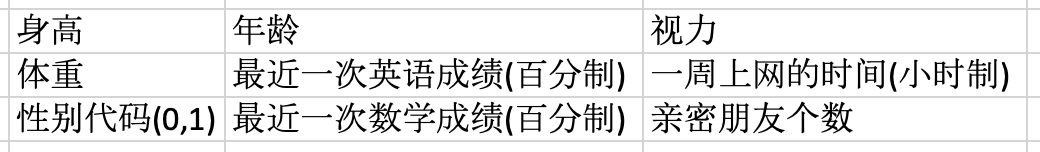
\includegraphics[width=0.7\textwidth]{fig/c3q2}
	\end{figure}
\end{question}
\noindent
提示:损失方程最简单就是,将矩阵的每个元素相减,然后求和。当然你也可以根据自己的喜好,对每个描述进行有比重的衡量。	根据你设计的损失方程,使用Python计算你与其它至少一位同学的相像值。
\end{fullmodel}


\begin{question}{作图题 C3-Q3}
	该题目具有承上启下的作用,虽然很简单,但是所蕴含的道理`法力无边'。给定方程$f(x) = -x^2+ 6x-2$, 下面是其图像,在这个图像中$x=2, x = 4, x =5$三个点上,画三条切线\mn{英文好的同学,可以阅读老师编写针对该问题的深入解释:\url{https://github.com/Michael-yunfei/MachineLearning/blob/master/GraidentDescent/Gradient.pdf}}。
	\begin{figure}[H]
		\centering
		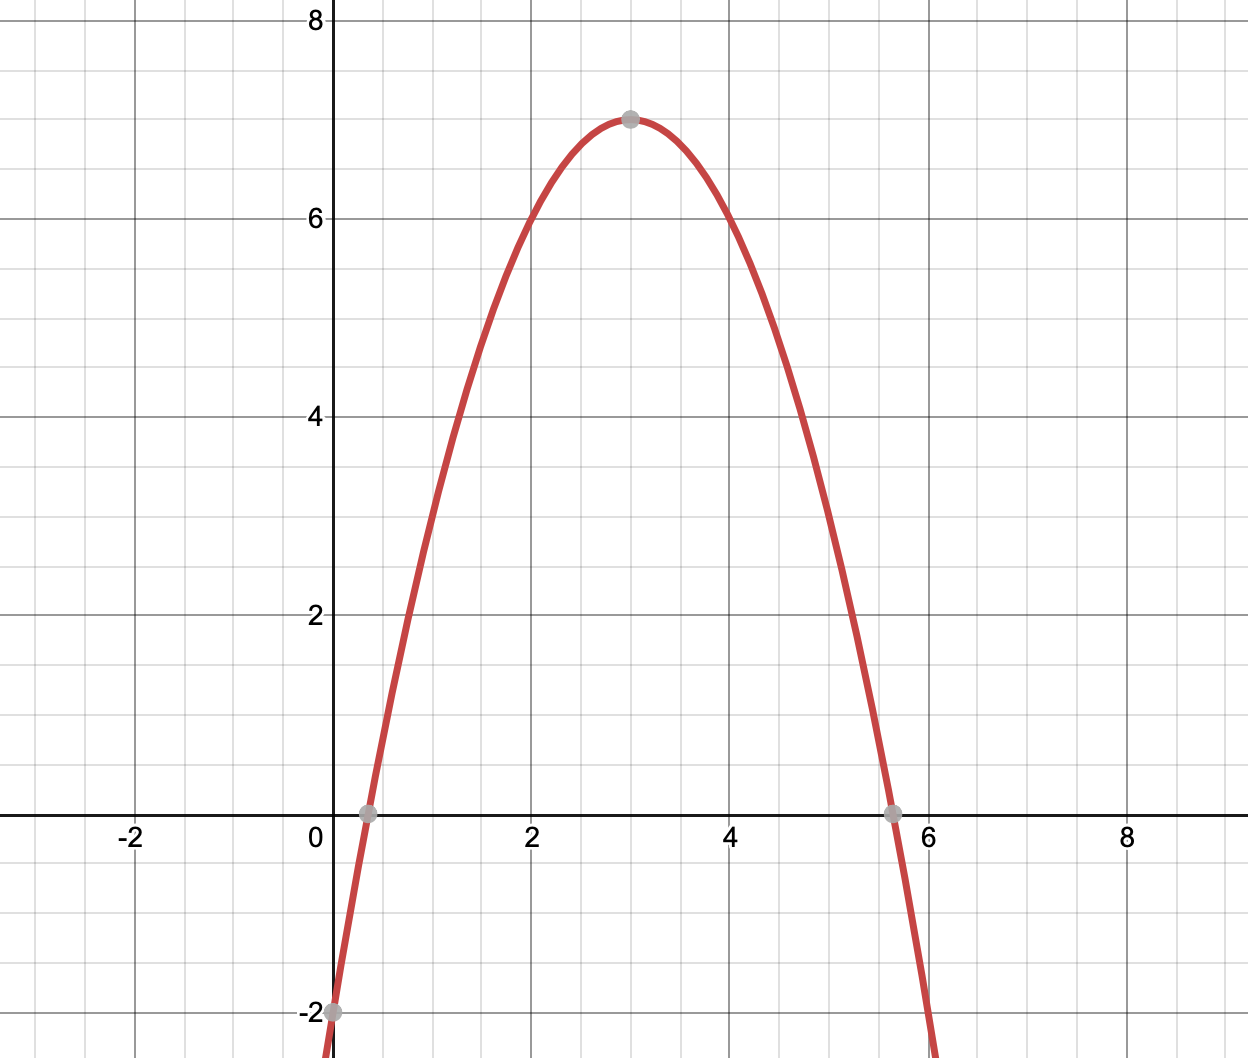
\includegraphics[width=0.6\textwidth]{fig/c3q3}
	\end{figure}
\end{question}


\begin{question}{计算题 C3-Q4}
	完成下列矩阵计算,请先手动计算,然后用Python计算。给定矩阵
	\begin{align*}
		A = \begin{bmatrix}
			3.2 & 1.7 \\
			5.1 & 8.9 
		\end{bmatrix}; \ \ \ B = \begin{bmatrix}
			0.9 & -1 \\
			 -1 & 0.1 
		\end{bmatrix}; \ \ \ C = \begin{bmatrix}
			2 & 3 & 9 \\
			7 & 8 & 6 \\
			1 & 0 & 5 
		\end{bmatrix}
	\end{align*}
	求矩阵的加法和卷积如下
	\begin{align*}
		A + B & = \ \ ? \\
		B * C &= \ \ ? \\
		B * A & = 
	\end{align*}
\end{question}


\noindent
khorosho(俄语,很好)!下节见。



\newpage
\part*{第四章:神经网络模型详解}





















\end{document}
